\documentclass[12pt, a4paper]{article}

% ==========================================
% 1. KHAI BÁO GÓI THƯ VIỆN (PACKAGES)
% ==========================================
% Bảng mã & Font chữ
\usepackage[utf8]{inputenc}
\usepackage[T5]{fontenc}

% Toán học
\usepackage{amsmath, amssymb}

% Căn lề & Bố cục trang
\usepackage[top=2.2cm, bottom=1.5cm, left=1cm, right=1cm, headheight=15pt]{geometry}
\usepackage{fancyhdr}
\usepackage{needspace}
\usepackage{tkz-tab}

% Đồ họa & Màu sắc
\usepackage{xcolor}
\usepackage{graphicx} 
\usepackage{tikz}
\usetikzlibrary{calc, shapes.geometric, positioning}


% Bảng biểu & Danh sách
\usepackage{colortbl}
\usepackage{array}
\usepackage{makecell}
\usepackage{multirow}
\usepackage{tasks}

% Biểu tượng
\usepackage{fontawesome5}

% ==========================================
% 2. THIẾT LẬP MÀU SẮC CHỦ ĐẠO
% ==========================================
\definecolor{goldyellow}{RGB}{255, 179, 0}
\definecolor{amberorange}{RGB}{230, 115, 0}
\definecolor{lightamber}{RGB}{255, 248, 225}
\definecolor{deepblue}{RGB}{25, 42, 86}
\definecolor{accentred}{RGB}{232, 65, 24}
\definecolor{softgray}{RGB}{220, 220, 222} 
\definecolor{fbblue}{RGB}{15, 80, 200}


% ==========================================
% 3. CẤU HÌNH HEADER & FOOTER
% ==========================================
\pagestyle{fancy}
\fancyhf{}
\renewcommand{\headrulewidth}{0pt}

% Khai báo biến lưu trữ nội dung góc phải của Header
\newcommand{\HeaderRightText}{}

% --- Header ---
\fancyhead[C]{
    \begin{tikzpicture}[remember picture, overlay]
        
        % Dải màu trang trí góc trên
        \path[fill=deepblue] (current page.north west) -- (current page.north east) 
            -- ($(current page.north east) + (0, -1.6cm)$) 
            .. controls ($(current page.north) + (3, -2.0cm)$) and ($(current page.north) + (-3, -0.4cm)$) .. 
            ($(current page.north west) + (0, -1.0cm)$) -- cycle;
            
        \path[fill=goldyellow] (current page.north west) -- (current page.north east) 
            -- ($(current page.north east) + (0, -1.0cm)$) 
            .. controls ($(current page.north) + (4, -1.0cm)$) and ($(current page.north) + (-2, -2.2cm)$) .. 
            ($(current page.north west) + (0, -1.6cm)$) -- cycle;
            
        \path[fill=amberorange] (current page.north west) -- ($(current page.north west) + (6.5cm, 0)$) 
            .. controls ($(current page.north west) + (4.5cm, -1.2cm)$) and ($(current page.north west) + (2cm, -2.0cm)$) .. 
            ($(current page.north west) + (0, -2.0cm)$) -- cycle;
            
        % Logo góc trái Header
        \node[anchor=west, inner sep=0pt] 
            at ($(current page.north west) + (0cm, -0.8cm)$) {\includegraphics[height=2.0cm]{../../image/logo-header.png}};
            
        % Text góc phải Header (Tự động lấy từ đối số thứ 3 của \titlebox)
        \node[anchor=east, text=white, font=\small\bfseries\sffamily] 
            at ($(current page.north east) + (-0.8cm, -0.5cm)$) {\HeaderRightText};
    \end{tikzpicture}
}

% --- Footer ---
\fancyfoot[C]{
    \begin{tikzpicture}[remember picture, overlay]
        % Đường kẻ ngang
        \draw[amberorange, line width=1.5pt] 
            ($(current page.south west) + (0cm, 0.4cm)$) -- ($(current page.south east) + (0cm, 0.4cm)$);

        % Dải cong góc phải
        \path[fill=goldyellow] (current page.south east) -- ($(current page.south east) + (-5cm, 0)$) 
            .. controls ($(current page.south east) + (-3cm, 0.8cm)$) and ($(current page.south east) + (-1.5cm, 1.2cm)$) .. 
            ($(current page.south east) + (0, 1.2cm)$) -- cycle;

        % Mạng xã hội
        \node[anchor=west, inner sep=0pt] at ($(current page.south west) + (1cm, 0.8cm)$) {
            \small\sffamily
            \textcolor{fbblue}{\faFacebook\hskip 4pt Toán Anh Huy MATH-STER}
            \hskip 18pt
            \textcolor{black}{\faTiktok\hskip 4pt huymathster}
        };

        % Số trang (Thiết kế hình tròn cũ thu nhỏ)
        \node[circle, fill=white, draw=amberorange, line width=1.5pt, text=deepblue, font=\large\bfseries, inner sep=0pt, minimum size=0.7cm] 
            at ($(current page.south east) + (-1.0cm, 0.65cm)$) {\thepage};
    \end{tikzpicture}
}

% ==========================================
% 4. ĐỊNH NGHĨA MACRO: KHUNG TIÊU ĐỀ
% ==========================================
\newcommand{\titlebox}[3]{
    % Gán nội dung đối số #3 vào biến HeaderRightText
    \gdef\HeaderRightText{#3}
    
    \begin{center}
    \vspace*{-0.5cm}
    \begin{tikzpicture}
        % Khung vô hình (Phantom Box) định chuẩn kích thước
        \node[text width=16cm, inner xsep=0pt, inner ysep=16pt, opacity=0] (MainBox) {
            \begin{minipage}[c]{4.2cm}
                \centering\vspace{0.1cm}
                \rule{2.2cm}{2.2cm} 
                \vspace{0.1cm}
            \end{minipage}%
            \begin{minipage}[c]{11.5cm}
                \centering\vspace{0.15cm}
                {\huge\bfseries\sffamily #2 \par}
                \vspace{0.15cm} 
            \end{minipage}
        };
        
        % Đổ bóng & Nền
        \fill[goldyellow, rounded corners=8pt] ([xshift=5pt, yshift=-5pt]MainBox.south west) rectangle ([xshift=5pt, yshift=-5pt]MainBox.north east);
        \fill[white, rounded corners=8pt] (MainBox.south west) rectangle (MainBox.north east);
        
        % Lưới ô ly & Nền Logo
        \begin{scope}
            \clip[rounded corners=8pt] (MainBox.south west) rectangle (MainBox.north east);
            \draw[step=0.4cm, softgray!50, line width=0.6pt] (MainBox.south west) grid (MainBox.north east);
            \fill[lightamber!60] (MainBox.south west) rectangle ([xshift=4.2cm]MainBox.north west);
        \end{scope}

        % Viền ngoài
        \draw[deepblue, line width=1.5pt, rounded corners=8pt] (MainBox.south west) rectangle (MainBox.north east);

        % Nội dung Text (Lớp trên cùng)
        \node[text width=16cm, inner xsep=0pt, inner ysep=16pt] at (MainBox.center) {
            \begin{minipage}[c]{4.2cm}
                \centering
                % --- ĐIỀU CHỈNH TỌA ĐỘ LOGO Ở ĐÂY ---
                \hspace*{-0.5cm}\raisebox{-0.2cm}{\includegraphics[width=5.5cm]{../../image/logo.png}}
            \end{minipage}%
            \begin{minipage}[c]{11.5cm}
                \centering\vspace{0.15cm}
                {\huge\bfseries\sffamily\color{deepblue} #2 \par}
                \vspace{0.15cm} 
            \end{minipage}
        };
        
        % Trang trí phụ kiện
        \draw[deepblue, line width=1.5pt, dashed] ([xshift=4.2cm]MainBox.north west) -- ([xshift=4.2cm]MainBox.south west);
        \node[regular polygon, regular polygon sides=4, rotate=45, fill=white, draw=accentred, line width=1.2pt, inner sep=2.5pt] at ([xshift=4.2cm]MainBox.west) {};
        \node[anchor=west, fill=amberorange, text=white, font=\large\bfseries\sffamily, rounded corners=4pt, draw=deepblue, line width=1.5pt, inner xsep=12pt, inner ysep=6pt] at ([xshift=1.5cm]MainBox.north west) {#1};
        \fill[accentred] ([xshift=-1.8cm, yshift=-0.4cm]MainBox.north east) circle (3pt);
        \fill[amberorange] ([xshift=-1.4cm, yshift=-0.4cm]MainBox.north east) circle (3pt);
        \fill[goldyellow] ([xshift=-1.0cm, yshift=-0.4cm]MainBox.north east) circle (3pt);
    \end{tikzpicture}
    \vspace*{0cm}
    \end{center}
}

% ==========================================
% 5. ĐỊNH NGHĨA MACRO: CẤU TRÚC CÂU HỎI (ÉP SÁT NHAU)
% ==========================================
\newcommand{\questioncore}[2]{
    % Xóa khoảng cách phía trên, ép sát câu trước
    \noindent \textbf{\textcolor{deepblue}{Câu #1.} \textcolor{accentred}{[STER]}} #2
    \par\nopagebreak
}

% Cấu hình hiển thị đáp án trắc nghiệm
\settasks{
    label=\textbf{\textcolor{amberorange}{\Alph*.}}, 
    label-width=15pt,     
    item-indent=25pt,     
    label-offset=6pt,    
    column-sep=20pt,     
    after-item-skip=2pt  % Đã giảm tối đa khoảng cách giữa các dòng đáp án A B C D
}

% Hàm vẽ dòng kẻ nháp
\newcommand{\drawdashlines}[1]{
    \ifnum#1>0
        \nopagebreak\vspace{0.1cm}\noindent 
        \begin{tikzpicture}
            \foreach \i in {1,...,#1} {
                \draw[softgray, line width=0.2pt] (0,-{\i*0.65}) -- (\textwidth-4pt,-{\i*0.65});
            }
        \end{tikzpicture}
        \par
    \fi
    % Đã xóa hoàn toàn khoảng cách thừa ở nhánh else
}

% --- Dạng 1: Trắc nghiệm 4 đáp án ---
\newcommand{\questionLinesManual}[4]{
    \pgfmathsetmacro{\calculatedSpace}{1.5 + #1 * 0.65}
    \needspace{\calculatedSpace cm} 
    \questioncore{#2}{#3}
    #4
    \par\nopagebreak
    \drawdashlines{#1}
}

% --- Dạng 2: Trắc nghiệm Đúng/Sai ---
\newcommand{\questionTrueFalse}[4]{
    \pgfmathsetmacro{\calculatedSpace}{3.0 + #1 * 0.65} 
    \needspace{\calculatedSpace cm}
    \questioncore{#2}{#3}
    
    \nopagebreak
    \begin{center}
    \renewcommand{\arraystretch}{1.2} % Bóp nhỏ chiều cao của bảng Đ/S
    \begin{tabular}{|>{\centering\arraybackslash}m{0.8cm}|m{12cm}|>{\centering\arraybackslash}m{2cm}|>{\centering\arraybackslash}m{2cm}|}
        \hline
        \rowcolor{amberorange!20}
        & \multicolumn{1}{>{\centering\arraybackslash}m{12cm}|}{\textbf{\textcolor{deepblue}{Mệnh đề}}} & 
        \textbf{\textcolor{deepblue}{Đúng}} & 
        \textbf{\textcolor{deepblue}{Sai}} \\
        \hline
        #4
        \hline
    \end{tabular}
    \renewcommand{\arraystretch}{1}
    \end{center}
    
    \par\nopagebreak
    \drawdashlines{#1}
}

% ----- Dạng 3: Tự luận ngắn -----
\newcommand{\questionShortAnswer}[3]{
    \pgfmathsetmacro{\calculatedSpace}{1.5 + #1 * 0.8}
    \needspace{\calculatedSpace cm}
    
    {\linespread{1.1}\selectfont % Bóp nhỏ giãn dòng của câu tự luận
    \questioncore{#2}{#3}\par}
    
    \nopagebreak
    \begin{flushright}
        \begin{tikzpicture}
            \node[anchor=east, font=\small\bfseries\sffamily, text=deepblue] 
                at (-0.2, 0.4) {Đáp án:};
            \fill[goldyellow, rounded corners=3pt] (0.08, -0.08) rectangle (3.08, 0.72);
            \draw[draw=deepblue, fill=white, line width=1.2pt, rounded corners=3pt] 
                (0,0) rectangle (3.0, 0.8);
            \foreach \x in {0.75, 1.5, 2.25} {
                \draw[draw=deepblue, line width=0.6pt] (\x, 0) -- (\x, 0.8);
            }
        \end{tikzpicture}
    \end{flushright}
    
    \par\nopagebreak
    \drawdashlines{#1}
}

% ==========================================
% BẮT ĐẦU NỘI DUNG TÀI LIỆU
% ==========================================
\begin{document}

% Truyền 3 tham số: {Nhãn cam} {Chữ to chính giữa} {Chữ ở góc phải Header}
\titlebox{Chủ đề: Hàm số}{Tính đơn điệu của hàm số}{Hàm số: Tính đơn điệu}

\questionLinesManual{0}{1}{ Cho hàm số \( f(x) \) có bảng biến thiên như sau:

\begin{center}
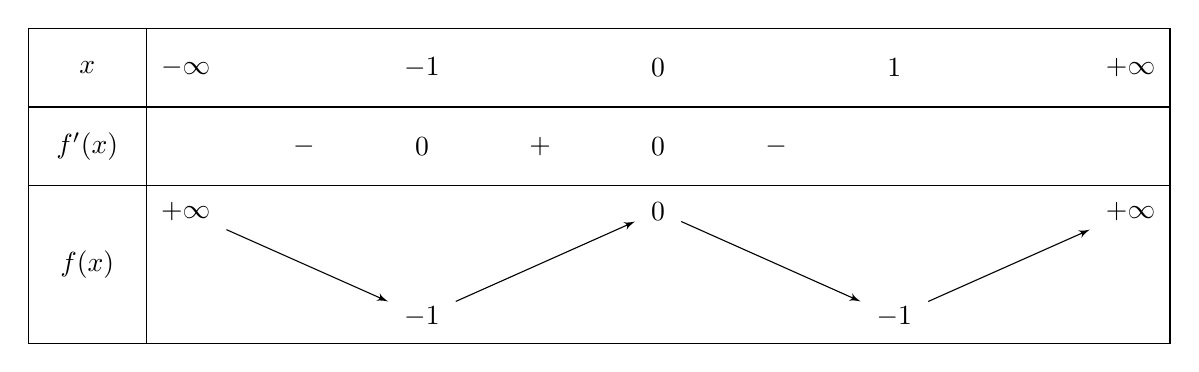
\begin{tikzpicture}
\tkzTabInit[color, lgt=1.5, espcl=3]  % <--- espcl là khoảng cách cột (tăng số này để bảng rộng hơn)
{$x$ / 1, $f'(x)$ / 1, $f(x)$ / 2}
{$-\infty$, $-1$, $0$, $1$, $+\infty$}
\tkzTabLine{ , -, 0, +, 0, - }
\tkzTabVar{+/$+\infty$, -/$-1$, +/$0$, -/$-1$, +/$+\infty$}
\end{tikzpicture}
\end{center}

Hàm số đã cho đồng biến trên khoảng nào dưới đây?}{%
\begin{tasks}(4)
\task \((-\infty; -1)\)
\task \((0; 1)\)
\task \((-1; 1)\)
\task \((-1; 0)\)
\end{tasks}
}
% ====== CÂU 2 ======
\questionLinesManual{0}{2}{Cho hàm số \( f(x) \) có bảng biến thiên như sau:
\begin{center}
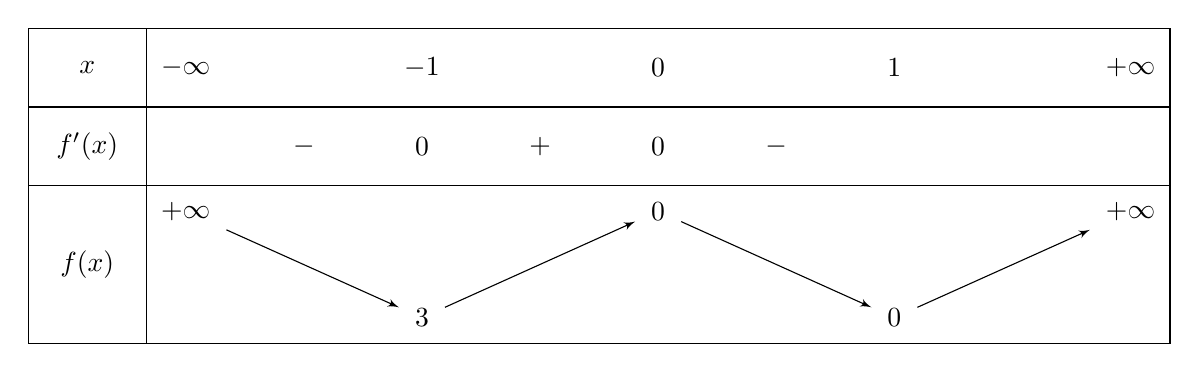
\begin{tikzpicture}
\tkzTabInit[color, lgt=1.5, espcl=3]
{$x$ / 1, $f'(x)$ / 1, $f(x)$ / 2}
{$-\infty$, $-1$, $0$, $1$, $+\infty$}
\tkzTabLine{ , -, 0, +, 0, - }
\tkzTabVar{+/$+\infty$, -/$3$, +/$0$, -/$0$, +/$+\infty$}
\end{tikzpicture}
\end{center}
Hàm số đã cho đồng biến trên khoảng nào sau đây?}{%
\begin{tasks}(4)
\task \((-\infty; -1)\)
\task \((0; 1)\)
\task \((-1; 0)\)
\task \((-1; +\infty)\)
\end{tasks}
}

% ====== CÂU 3 ======
\questionLinesManual{0}{3}{Cho hàm số \( y = f(x) \) có bảng xét dấu đạo hàm như sau:
\begin{center}
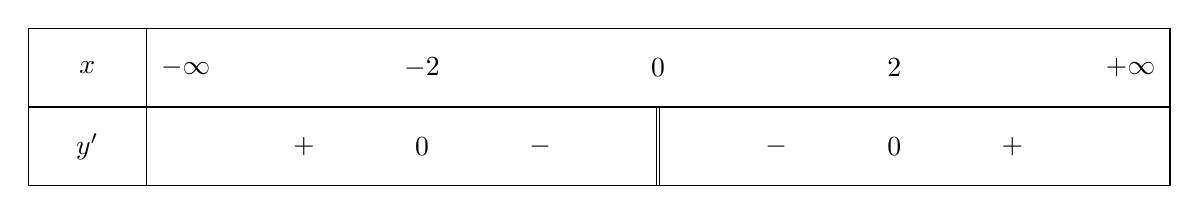
\begin{tikzpicture}
\tkzTabInit[color, lgt=1.5, espcl=3]
{$x$ / 1, $y'$ / 1}
{$-\infty$, $-2$, $0$, $2$, $+\infty$}
\tkzTabLine{ , +, 0, -, d, -,0,+}
\end{tikzpicture}
\end{center}
Mệnh đề nào dưới đây đúng?}{%
\begin{tasks}(2)
\task Hàm số nghịch biến trên khoảng \((-\infty; -2)\).
\task Hàm số đồng biến trên khoảng \((-2; 0)\).
\task Hàm số đồng biến trên khoảng \((0; 2)\).
\task Hàm số nghịch biến trên khoảng \((0; 2)\).
\end{tasks}
}

% ====== CÂU 4 ======
\questionLinesManual{0}{4}{Cho hàm số \( y = f(x) \) có bảng xét dấu của đạo hàm như hình vẽ.
Hàm số đã cho nghịch biến trên khoảng nào dưới đây?
\begin{center}
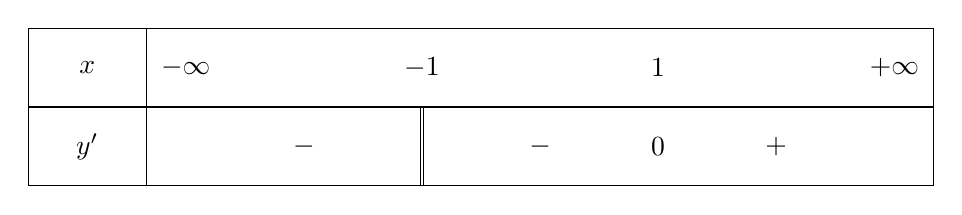
\begin{tikzpicture}
\tkzTabInit[color, lgt=1.5, espcl=3]
{$x$ / 1, $y'$ / 1}
{$-\infty$, $-1$, $1$, $+\infty$}
\tkzTabLine{ , -, d, -, 0 ,+}
\end{tikzpicture}
\end{center}}{%
\begin{tasks}(4)
\task \((1; +\infty)\)
\task \((-\infty; 1)\)
\task \((-1; +\infty)\)
\task \((-\infty; -1)\)
\end{tasks}
}

% ====== CÂU 5 ======
\questionLinesManual{0}{5}{Cho hàm số \( y = f(x) \) có bảng biến thiên như hình dưới đây. Mệnh đề nào sau đây là đúng?
\begin{center}
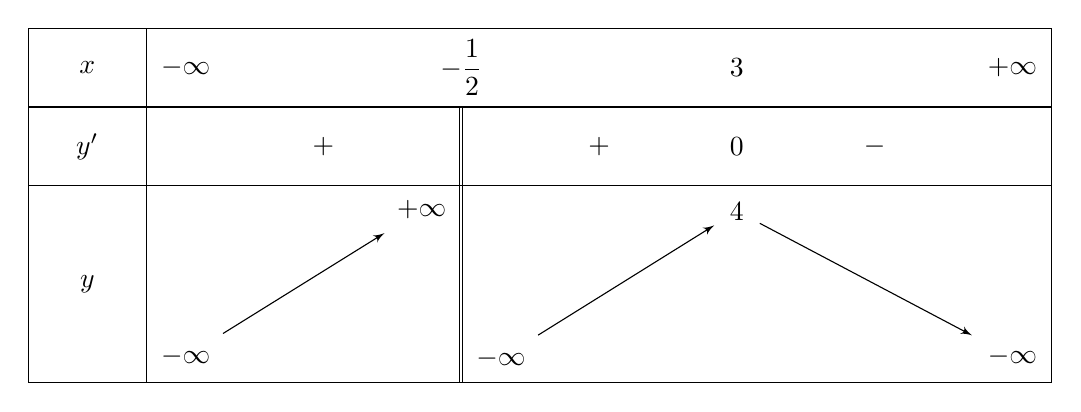
\begin{tikzpicture}
\tkzTabInit[color, lgt=1.5, espcl=3.5]
{$x$ / 1, $y'$ / 1, $y$ / 2.5}
{$-\infty$, $-\dfrac{1}{2}$, $3$, $+\infty$}
\tkzTabLine{ , +, d, +, 0, - , }
\tkzTabVar{-/ $-\infty$, +D-/ $+\infty$ / $-\infty$, +/ $4$, -/ $-\infty$}
\end{tikzpicture}
\end{center}}{%
\begin{tasks}(1)
\task Hàm số đã cho đồng biến trên khoảng \( \left( -\dfrac{1}{2}; +\infty \right) \).
\task Hàm số đã cho đồng biến trên khoảng \( (-\infty; 3) \).
\task Hàm số đã cho nghịch biến trên khoảng \( (3; +\infty) \).
\task Hàm số đã cho nghịch biến trên các khoảng \( \left( -\infty; -\dfrac{1}{2} \right) \) và \( (3; +\infty) \).
\end{tasks}
}

% ====== CÂU 6 ======
% ====== CÂU 6 ======
\questionLinesManual{0}{6}{Cho hàm số \( f(x) \) có bảng biến thiên như sau:
\begin{center}
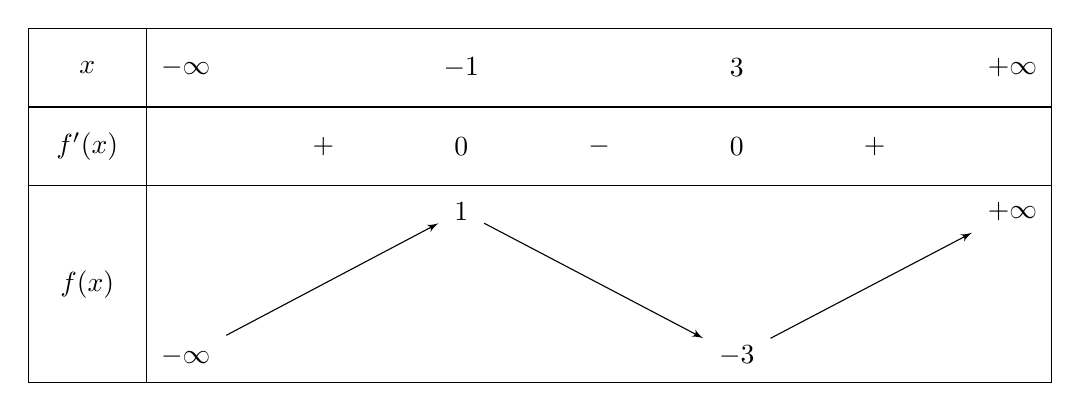
\begin{tikzpicture}
\tkzTabInit[color, lgt=1.5, espcl=3.5]
{$x$ / 1, $f'(x)$ / 1, $f(x)$ / 2.5}
{$-\infty$, $-1$, $3$, $+\infty$}
\tkzTabLine{ , +, 0, -, 0, + }
\tkzTabVar{-/$-\infty$, +/$1$, -/$-3$, +/$+\infty$}
\end{tikzpicture}
\end{center}
Hàm số đã cho đồng biến trên khoảng nào sau đây?}{%
\begin{tasks}(4)
\task \( (-\infty; 1) \)
\task \( (3; +\infty) \)
\task \( (-1; 3) \)
\task \( (-3; +\infty) \)
\end{tasks}
}
% ====== CÂU 7 ======
\questionLinesManual{0}{7}{Cho hàm số \( y = f(x) \) liên tục trên \( \mathbb{R} \) có bảng xét dấu \( f'(x) \) cho như hình vẽ.
\begin{center}
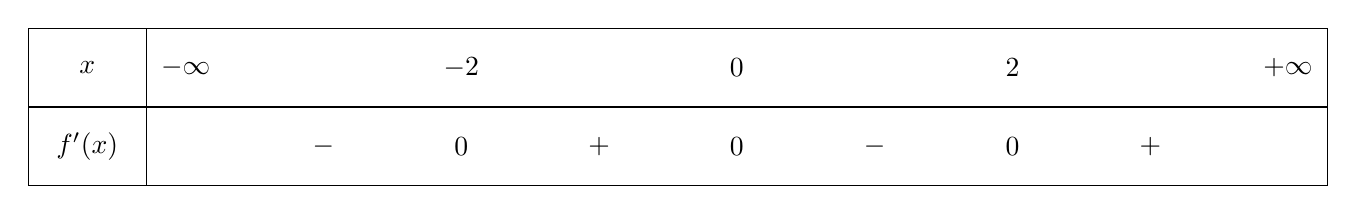
\begin{tikzpicture}
\tkzTabInit[color, lgt=1.5, espcl=3.5]
{$x$ / 1, $f'(x)$ / 1}
{$-\infty$, $-2$, $0$, $2$, $+\infty$}
\tkzTabLine{ , -, 0, +, 0, -,0,+} 
\end{tikzpicture}
\end{center}
Hàm số đã cho nghịch biến trên khoảng nào dưới đây?}{%
\begin{tasks}(4)
\task \( (2; +\infty) \)
\task \( (-2; 0) \)
\task \( (-\infty; 0) \)
\task \( (0; 2) \)
\end{tasks}
}

% ====== CÂU 8 ======
\questionLinesManual{0}{8}{Cho hàm số \( f(x) \) có bảng biến thiên như sau:
\begin{center}
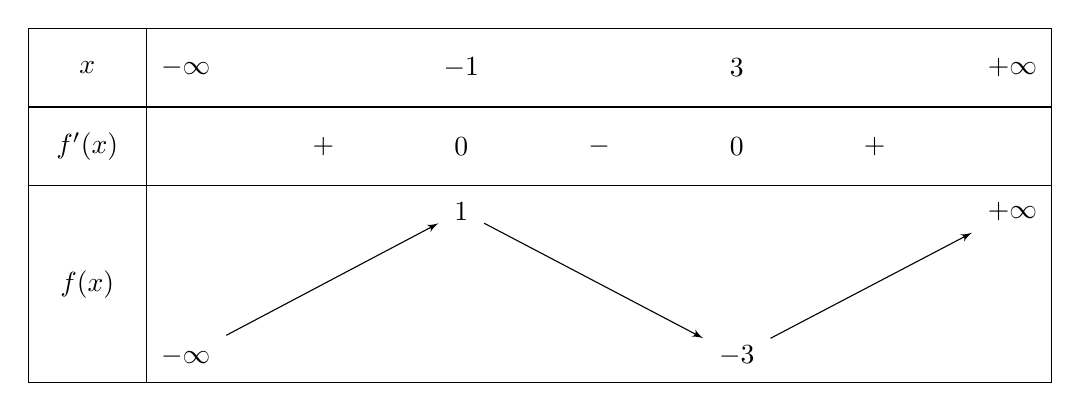
\begin{tikzpicture}
\tkzTabInit[color, lgt=1.5, espcl=3.5]
{$x$ / 1, $f'(x)$ / 1, $f(x)$ / 2.5}
{$-\infty$, $-1$, $3$, $+\infty$}
\tkzTabLine{ , +, 0, -, 0, + }
\tkzTabVar{-/$-\infty$, +/$1$, -/$-3$, +/$+\infty$}
\end{tikzpicture}
\end{center}
Hàm số đã cho đồng biến trên khoảng nào sau đây?}{%
\begin{tasks}(4)
\task \( (-\infty; 1) \)
\task \( (3; +\infty) \)
\task \( (-1; 3) \)
\task \( (-3; +\infty) \)
\end{tasks}
}

% ====== CÂU 9 ======
\questionLinesManual{0}{9}{Cho hàm số \( y = f(x) \) có bảng biến thiên như sau:
\begin{center}
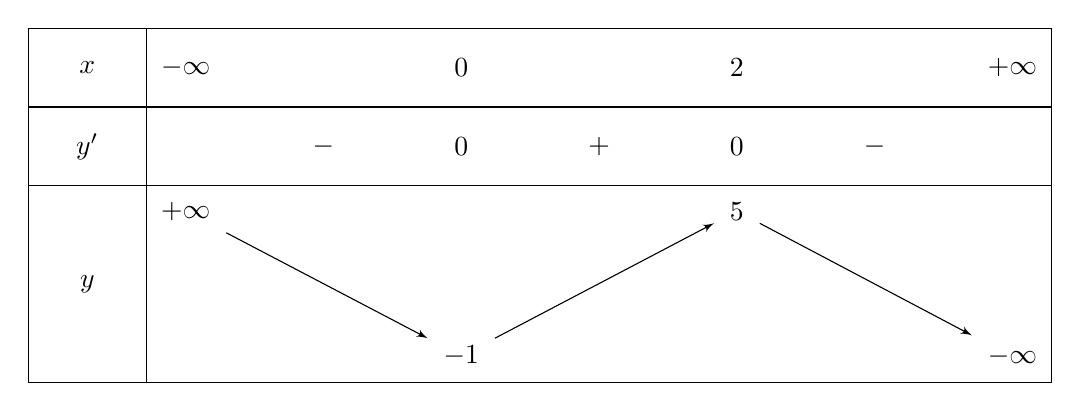
\begin{tikzpicture}
\tkzTabInit[color, lgt=1.5, espcl=3.5]
{$x$ / 1, $y'$ / 1, $y$ / 2.5}
{$-\infty$, $0$, $2$, $+\infty$}
\tkzTabLine{ , -, 0, +, 0, - }
\tkzTabVar{+/$+\infty$, -/$-1$, +/$5$, -/$-\infty$}
\end{tikzpicture}
\end{center}
Hàm số đã cho nghịch biến trên khoảng nào dưới đây?}{%
\begin{tasks}(4)
\task \( (-\infty; 2) \)
\task \( (0; 2) \)
\task \( (0; +\infty) \)
\task \( (3; 2024) \)
\end{tasks}
}

% ====== CÂU 10 ======
\questionLinesManual{0}{10}{Cho hàm số \( y = f(x) \) liên tục trên \( \mathbb{R} \) có bảng xét dấu \( f'(x) \) cho như hình vẽ.
\begin{center}
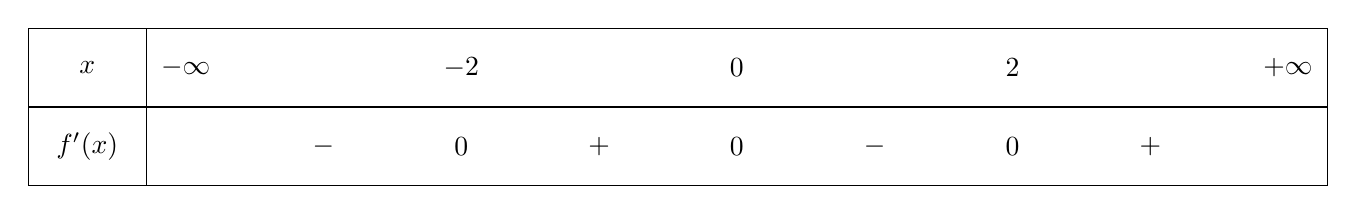
\begin{tikzpicture}
\tkzTabInit[color, lgt=1.5, espcl=3.5]
{$x$ / 1, $f'(x)$ / 1}
{$-\infty$, $-2$, $0$, $2$, $+\infty$}
\tkzTabLine{ , -, 0, +, 0, - ,0,+}
\end{tikzpicture}
\end{center}
Hàm số đã cho nghịch biến trên khoảng nào dưới đây?}{%
\begin{tasks}(4)
\task \( (2; +\infty) \)
\task \( (-2; 0) \)
\task \( (-\infty; 0) \)
\task \( (0; 2) \)
\end{tasks}
}

% ====== CÂU 11 ======
\questionLinesManual{0}{11}{Cho hàm số \( f(x) \) có bảng biến thiên như sau:
\begin{center}
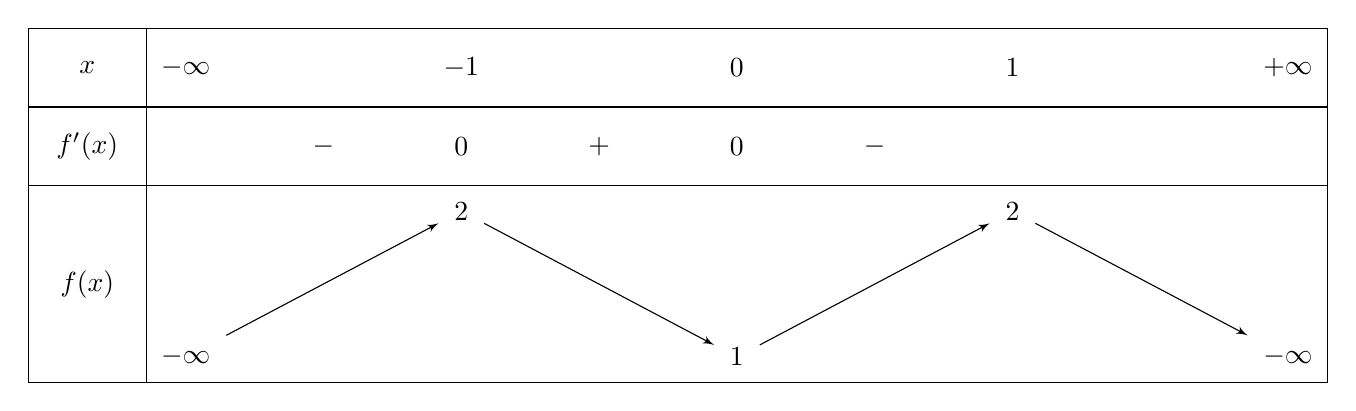
\begin{tikzpicture}
\tkzTabInit[color, lgt=1.5, espcl=3.5]
{$x$ / 1, $f'(x)$ / 1, $f(x)$ / 2.5}
{$-\infty$, $-1$, $0$, $1$, $+\infty$}
\tkzTabLine{ , -, 0, +, 0, - }
\tkzTabVar{-/$-\infty$, +/$2$, -/$1$, +/$2$, -/$-\infty$}
\end{tikzpicture}
\end{center}
Hàm số đã cho nghịch biến trên khoảng nào dưới đây?}{%
\begin{tasks}(4)
\task \((-\infty; -1)\)
\task \((0; 1)\)
\task \((-1; 0)\)
\task \((-\infty; 0)\)
\end{tasks}
}

% ====== CÂU 12 ======
\questionLinesManual{0}{12}{Cho hàm số \( y = f(x) \) có bảng biến thiên như sau:
\begin{center}
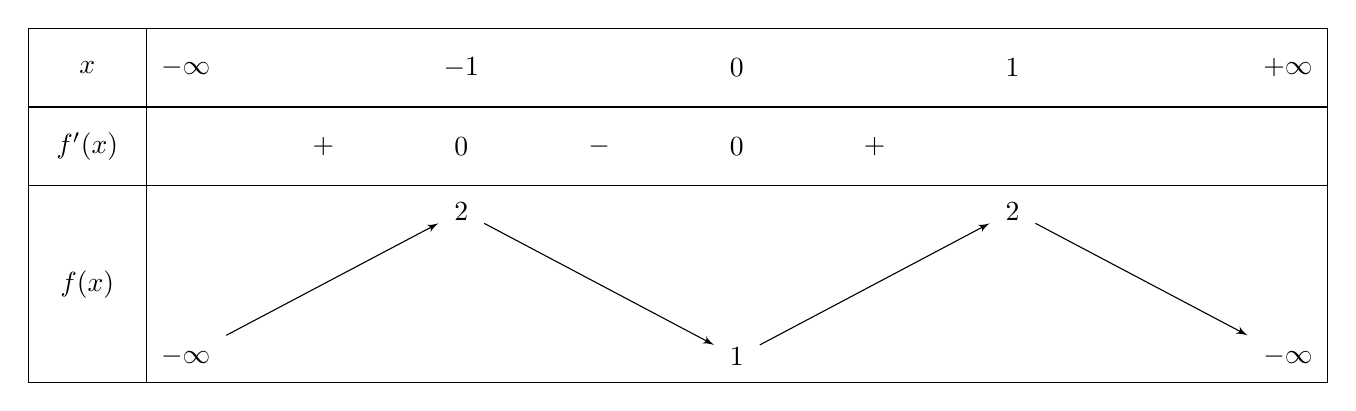
\begin{tikzpicture}
\tkzTabInit[color, lgt=1.5, espcl=3.5]
{$x$ / 1, $f'(x)$ / 1, $f(x)$ / 2.5}
{$-\infty$, $-1$, $0$, $1$, $+\infty$}
\tkzTabLine{ , +, 0, -, 0, + }
\tkzTabVar{-/$-\infty$, +/$2$, -/$1$, +/$2$, -/$-\infty$}
\end{tikzpicture}
\end{center}
Hàm số đã cho đồng biến trên khoảng nào dưới đây?}{%
\begin{tasks}(4)
\task \((1; +\infty)\)
\task \((-1; 0)\)
\task \((-1; 1)\)
\task \((0; 1)\)
\end{tasks}
}

% ====== CÂU 13 ======
\questionLinesManual{0}{13}{Cho hàm số \( f(x) \) có bảng biến thiên như sau:
\begin{center}
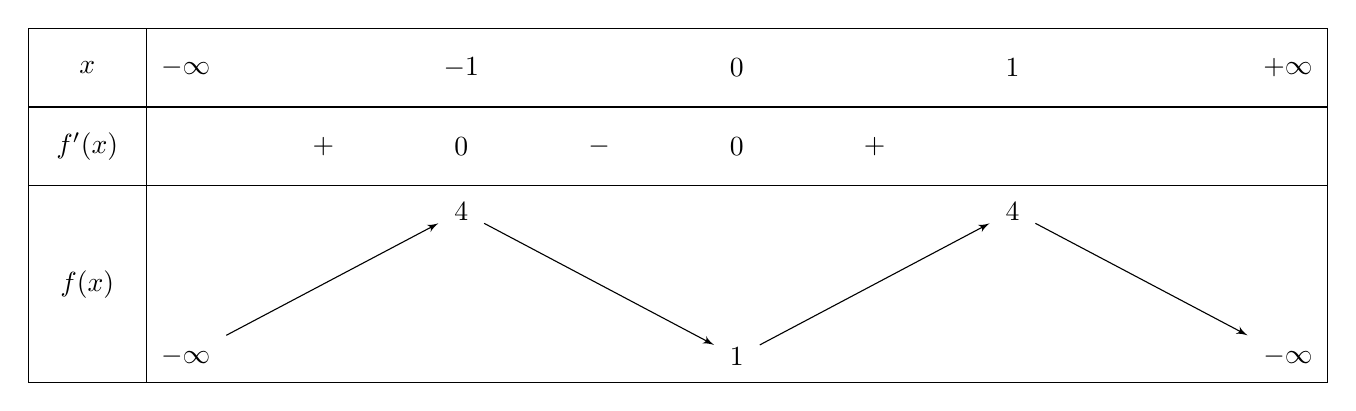
\begin{tikzpicture}
\tkzTabInit[color, lgt=1.5, espcl=3.5]
{$x$ / 1, $f'(x)$ / 1, $f(x)$ / 2.5}
{$-\infty$, $-1$, $0$, $1$, $+\infty$}
\tkzTabLine{ , +, 0, -, 0, + }
\tkzTabVar{-/$-\infty$, +/$4$, -/$1$, +/$4$, -/$-\infty$}
\end{tikzpicture}
\end{center}
Hàm số đã cho đồng biến trên khoảng nào dưới đây?}{%
\begin{tasks}(4)
\task \((1; +\infty)\)
\task \((-1; 1)\)
\task \((0; 1)\)
\task \((-1; 0)\)
\end{tasks}
}

% ====== CÂU 14 (hoặc 15 theo ảnh) ======
\questionLinesManual{0}{14}{Cho hàm số \( f(x) \) có bảng biến thiên như sau:
\begin{center}
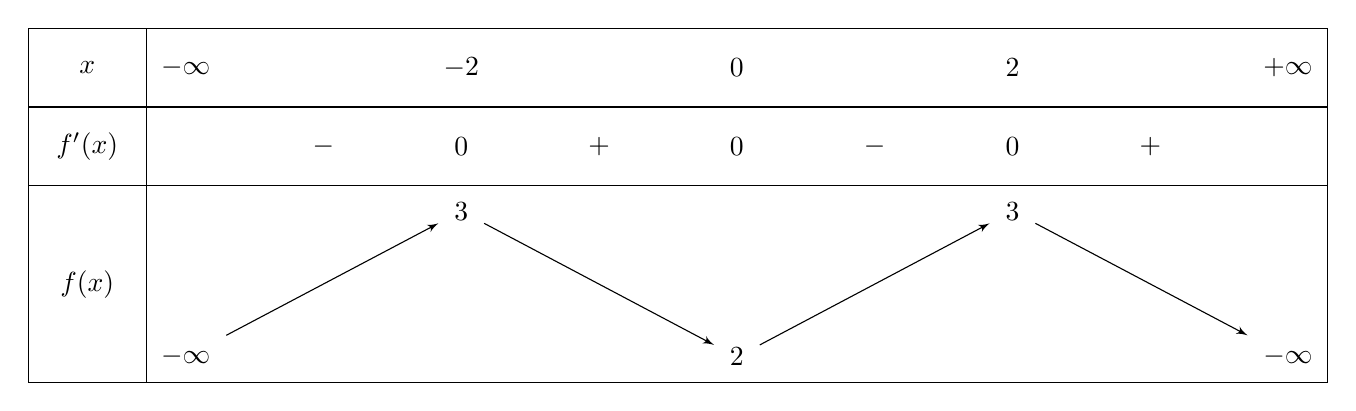
\begin{tikzpicture}
\tkzTabInit[color, lgt=1.5, espcl=3.5]
{$x$ / 1, $f'(x)$ / 1, $f(x)$ / 2.5}
{$-\infty$, $-2$, $0$, $2$, $+\infty$}
\tkzTabLine{ , -, 0, +, 0, -, 0, + }
\tkzTabVar{-/$-\infty$, +/$3$, -/$2$, +/$3$, -/$-\infty$}
\end{tikzpicture}
\end{center}
Hàm số đã cho đồng biến trên khoảng nào dưới đây?}{%
\begin{tasks}(4)
\task \((-2; 2)\)
\task \((0; 2)\)
\task \((-2; 0)\)
\task \((2; +\infty)\)
\end{tasks}
}

% ====== CÂU 15 ======
\questionLinesManual{0}{15}{Cho hàm số \( f(x) \) có bảng biến thiên như sau:
\begin{center}
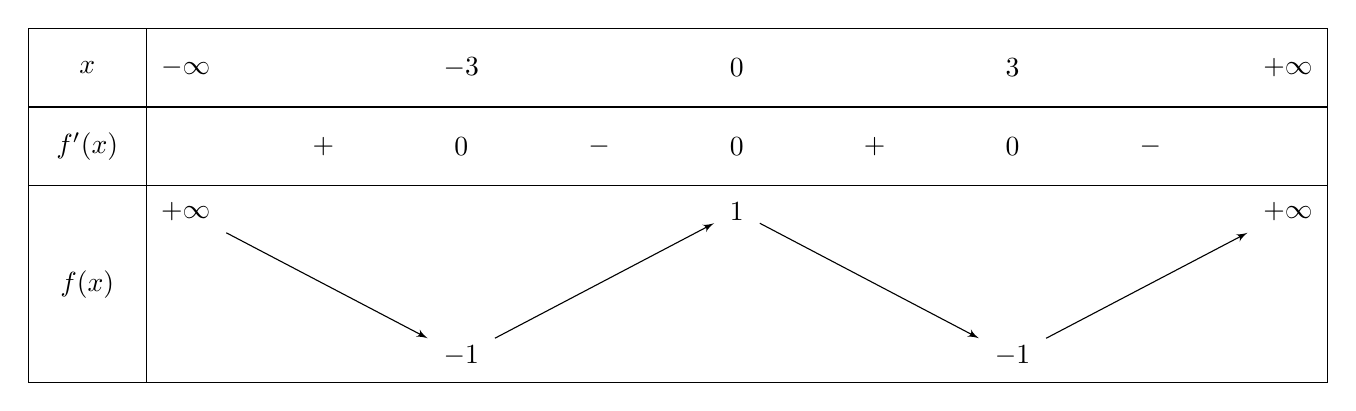
\begin{tikzpicture}
\tkzTabInit[color, lgt=1.5, espcl=3.5]
{$x$ / 1, $f'(x)$ / 1, $f(x)$ / 2.5}
{$-\infty$, $-3$, $0$, $3$, $+\infty$}
\tkzTabLine{ , +, 0, -, 0, +, 0, - }
\tkzTabVar{+/$+\infty$, -/$-1$, +/$1$, -/$-1$, +/$+\infty$}
\end{tikzpicture}
\end{center}
Hàm số đã cho đồng biến trên khoảng nào dưới đây?}{%
\begin{tasks}(4)
\task \((-3; 0)\)
\task \((-3; 3)\)
\task \((0; 3)\)
\task \((-\infty; -3)\)
\end{tasks}
}

% ====== CÂU 16 ======
\questionLinesManual{0}{16}{Cho hàm số \( y = f(x) \) có đồ thị là đường cong hình bên. Hàm số đã cho đồng biến trên khoảng nào dưới đây?
\begin{center}
\begin{tikzpicture}[>=latex, scale=1]
    % 1. Vẽ hệ trục tọa độ Ox, Oy
    \draw[->] (-2.5,0) -- (2.5,0) node[below] {\small $x$};
    \draw[->] (0,-1.7) -- (0,2.5) node[right] {\small $y$};
    \node[above left] at (0,0) {\small $O$};
    
    % 2. Vẽ đồ thị hàm số y = x^4 - 2x^2 chuẩn chỉnh
    % Dùng biểu thức thuần nhân (\x*\x*\x*\x) để tránh lỗi xử lý dấu ^ của TikZ
    \draw[thick, color=black!80, samples=150, domain=-1.6:1.6] 
        plot (\x, {\x*\x*\x*\x - 2*\x*\x}); 
        
    % 3. Vẽ các đường nét đứt gióng tọa độ cực trị (Đối xứng tuyệt đối)
    \draw[dashed] (-1,0) -- (-1,-1) -- (1,-1) -- (1,0);
    
    % 4. Điền nhãn số tại các điểm gióng
    \node[above ] at (-1,0) {\small $-1$};
    \node[above ] at (1,0) {\small $1$};
    \node[below left] at (0,-1) {\small $-1$};
\end{tikzpicture}
\end{center}}{%
\begin{tasks}(4)
\task \( (-1;0) \).
\task \( (-\infty;-1) \).
\task \( (0;+\infty) \).
\task \( (0;1) \).
\end{tasks}
}



% ====== CÂU 17 (Câu 23 trong ảnh gốc) ======
\questionLinesManual{0}{17}{Cho hàm số \( y = f(x) \) có đồ thị như hình vẽ bên. Hàm số đã cho đồng biến trên khoảng nào dưới đây?
\begin{center}
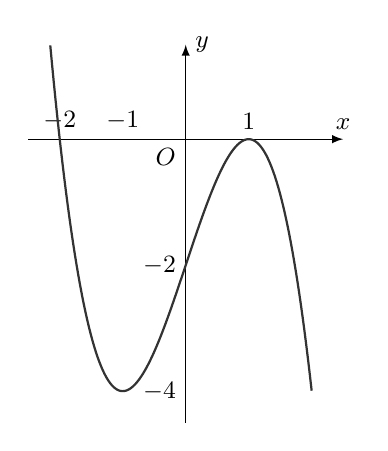
\begin{tikzpicture}[>=latex, scale=0.8]
    % Vẽ hệ trục tọa độ Ox, Oy
    \draw[->] (-2.5,0) -- (2.5,0) node[above] {\small $x$};
    \draw[->] (0,-4.5) -- (0,1.5) node[right] {\small $y$};
    \node[below left] at (0,0) {\small $O$};
    
    % Điền nhãn tọa độ trên trục chuẩn theo hình
    \node[above ] at (-2,0) {\small $-2$};
    \node[above ] at (-1,0) {\small $-1$};
    \node[above ] at (1,0) {\small $1$};
    \node[left] at (0,-2) {\small $-2$};
    \node[left] at (0,-4) {\small $-4$};
    
    % Vẽ đồ thị bằng hàm số chuẩn y = -x^3 + 3x - 2
    \draw[thick, color=black!80, samples=150, domain=-2.15:2] 
        plot (\x, {-\x*\x*\x + 3*\x - 2}); 
        
    
\end{tikzpicture}
\end{center}}{%
\begin{tasks}(4)
\task \((-\infty; -1)\).
\task \((-1; 1)\).
\task \((0; +\infty)\).
\task \((-\infty; +\infty)\).
\end{tasks}
}

% ====== CÂU 18 (Câu 24 trong ảnh) ======
\questionLinesManual{0}{18}{Cho hàm số \( y = f(x) \) có đồ thị như hình vẽ bên. Hàm số đã cho nghịch biến trên khoảng nào dưới đây?
\begin{center}
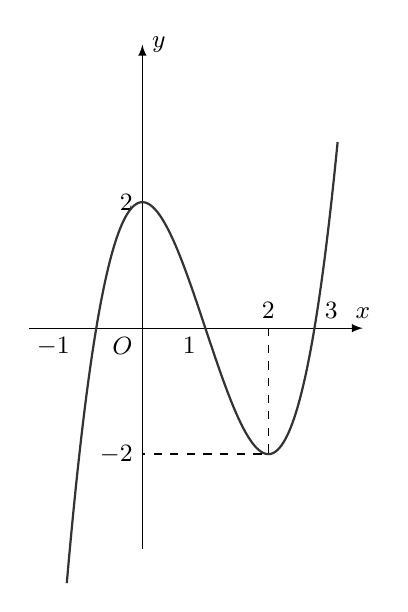
\begin{tikzpicture}[>=latex, scale=0.8]
    % Vẽ hệ trục tọa độ Ox, Oy
    \draw[->] (-1.8,0) -- (3.5,0) node[above] {\small $x$};
    \draw[->] (0,-3.5) -- (0,4.5) node[right] {\small $y$};
    \node[below left] at (0,0) {\small $O$};
    
    % Điền nhãn tọa độ trên trục
    \node[below left] at (-1,0) {\small $-1$};
    \node[below left] at (1,0) {\small $1$};
    \node[above] at (2,0) {\small $2$};
    \node[above] at (3,0) {\small $3$};
    \node[left] at (0,2) {\small $2$};
    
    % Vẽ đồ thị bằng hàm số chính xác y = x^3 - 3x^2 + 2
    \draw[thick, color=black!80, samples=150, domain=-1.2:3.1] 
        plot (\x, {\x*\x*\x - 3*\x*\x + 2}); 
        
    % Đường nét đứt gióng tọa độ cực tiểu (2; -2)
    \draw[dashed, line width=0.5pt] (2,0) -- (2,-2) -- (0,-2);
    \node[left] at (0,-2) {\small $-2$};
\end{tikzpicture}
\end{center}}{%
\begin{tasks}(4)
\task \((-1; 1)\).
\task \((-1; 2)\).
\task \((1; 2)\).
\task \((2; +\infty)\).
\end{tasks}
}

% ====== CÂU 19 (Câu 25 trong ảnh) ======
\questionLinesManual{0}{19}{Cho hàm số \( y = f(x) \) có đồ thị như hình vẽ bên. Hàm số đã cho nghịch biến trên khoảng nào dưới đây?
\begin{center}
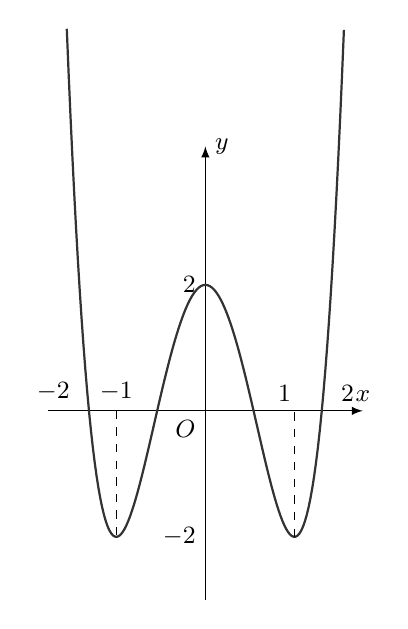
\begin{tikzpicture}[>=latex, scale=0.8]
    % Vẽ hệ trục tọa độ Ox, Oy
    \draw[->] (-2.5,0) -- (2.5,0) node[above] {\small $x$};
    \draw[->] (0,-3.0) -- (0,4.2) node[right] {\small $y$};
    \node[below left] at (0,0) {\small $O$};
    
    % Điền nhãn tọa độ chuẩn đi qua các điểm cắt Ox và Oy
    \node[above left] at (-2,0) {\small $-2$};
    \node[above left] at (-1,0) {\small $-1$};
    \node[above right] at (1,0) {\small $1$};
    \node[above right] at (2,0) {\small $2$};
    \node[left] at (0,2) {\small $2$};
    \node[left] at (0,-2) {\small $-2$};
    
    % Vẽ đồ thị dạng chữ W chuẩn bằng hàm y = x^4 - 4x^2 + 2
    \draw[thick, color=black!80, samples=150, domain=-2.2:2.2] 
        plot (\x, {\x*\x*\x*\x - 4*\x*\x + 2}); 
        
    % Đường nét đứt gióng từ cực tiểu (x = +-sqrt(2) = +-1.41) xuống y = -2 chuẩn chỉnh 100%
    \draw[dashed, line width=0.5pt] (-1.414, 0) -- (-1.414, -2) (1.414, -2) -- (1.414, 0);
\end{tikzpicture}
\end{center}}{%
\begin{tasks}(4)
\task \((-\infty; -1)\).
\task \((-1; 1)\).
\task \((1; 2)\).
\task \((0; 1)\).
\end{tasks}
}

% ====== CÂU 20 (Câu 26 trong ảnh) ======
\questionLinesManual{0}{20}{Cho hàm số \( y = f(x) \) có đồ thị như hình vẽ bên.
\begin{center}
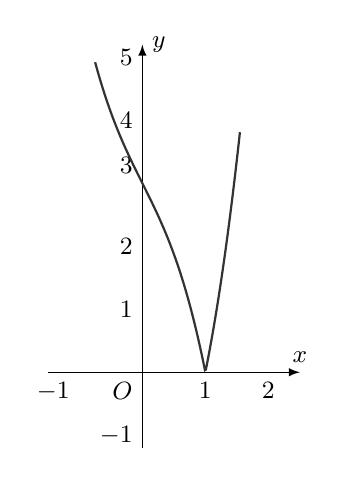
\begin{tikzpicture}[>=latex, scale=0.8]
    % Vẽ hệ trục tọa độ Ox, Oy
    \draw[->] (-1.5,0) -- (2.5,0) node[above] {\small $x$};
    \draw[->] (0,-1.2) -- (0,5.2) node[right] {\small $y$};
    \node[below left] at (0,0) {\small $O$};
    
    % Điền nhãn tọa độ trên trục
    \node[below left] at (-1,0) {\small $-1$};
    \node[below] at (1,0) {\small $1$};
    \node[below] at (2,0) {\small $2$};
    \node[left] at (0,-1) {\small $-1$};
    \node[left] at (0,1) {\small $1$};
    \node[left] at (0,2) {\small $2$};
    \node[above left] at (0,3) {\small $3$};
    \node[left] at (0,4) {\small $4$};
    \node[left] at (0,5) {\small $5$};
    
    % Vẽ đồ thị hàm số chuẩn xác bậc 3: y = 3x^3 - 3x^2 - 3x + 3
    \draw[thick, color=black!80, samples=150, domain=-0.75:1.55] 
        plot (\x, {abs(-\x*\x*\x - 2*\x + 3)}); 
\end{tikzpicture}
\end{center}
Mệnh đề nào sau đây là \textbf{đúng}?}{%
\begin{tasks}(1)
\task Hàm số đã cho đồng biến trên khoảng \((0;2)\).
\task Hàm số đã cho đồng biến trên khoảng \((-1;+\infty)\).
\task Hàm số đã cho nghịch biến trên khoảng \((-1;2)\).
\task Hàm số đã cho nghịch biến trên khoảng \((-\infty;1)\).
\end{tasks}
}

% ====== CÂU 21 (Câu 27 trong ảnh) ======
\questionLinesManual{0}{21}{Cho hàm số \( y = f(x) \) có đồ thị như hình vẽ bên. Hàm số đã cho đồng biến trên khoảng nào?
\begin{center}
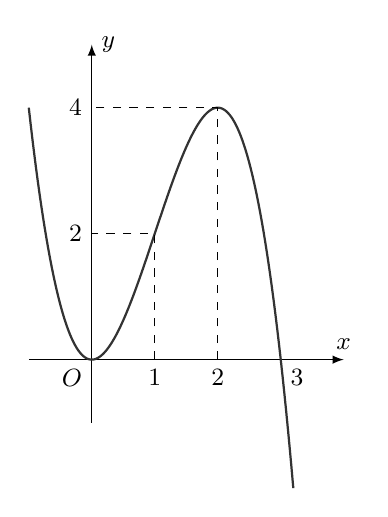
\begin{tikzpicture}[>=latex, scale=0.8]
    % Vẽ hệ trục tọa độ Ox, Oy
    \draw[->] (-1.0,0) -- (4.0,0) node[above] {\small $x$};
    \draw[->] (0,-1.0) -- (0,5.0) node[right] {\small $y$};
    \node[below left] at (0,0) {\small $O$};
    
    % Nhãn tọa độ
    \node[below] at (1,0) {\small $1$};
    \node[below] at (2,0) {\small $2$};
    \node[below right] at (3,0) {\small $3$};
    \node[left] at (0,2) {\small $2$};
    \node[left] at (0,4) {\small $4$};
    
    % Đồ thị hàm bậc 3: y = -x^3 + 3x^2
    \draw[thick, color=black!80, samples=150, domain=-1:3.2] 
        plot (\x, {-\x*\x*\x + 3*\x*\x}); 
        
    % Nét đứt gióng tọa độ cực đại (2;4) và điểm bổ trợ (1;2) chuẩn chỉnh
    \draw[dashed, line width=0.5pt] (2,0) -- (2,4) -- (0,4);
    \draw[dashed, line width=0.5pt] (1,0) -- (1,2) -- (0,2);
\end{tikzpicture}
\end{center}}{%
\begin{tasks}(4)
\task \((-\infty;0)\).
\task \((1;3)\).
\task \((0;2)\).
\task \((0;+\infty)\).
\end{tasks}
}

% ====== CÂU 22 (Câu 28 trong ảnh) ======
\questionLinesManual{0}{22}{Cho hàm số \( y = f(x) \) có đồ thị như hình vẽ bên. Hàm số đã cho nghịch biến trên khoảng nào?
\begin{center}
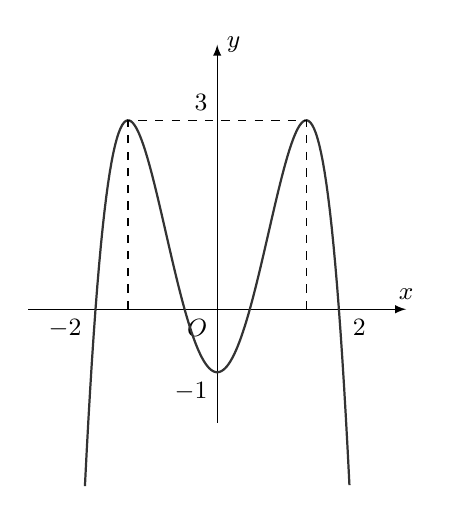
\begin{tikzpicture}[>=latex, scale=0.8]
    % Vẽ hệ trục tọa độ Ox, Oy
    \draw[->] (-3.0,0) -- (3.0,0) node[above] {\small $x$};
    \draw[->] (0,-1.8) -- (0,4.2) node[right] {\small $y$};
    \node[below left] at (0,0) {\small $O$};
    
    % Nhãn tọa độ
    \node[below left] at (-2,0) {\small $-2$};
    \node[below right] at (2,0) {\small $2$};
    \node[below left] at (0,-1) {\small $-1$};
    \node[above left] at (0,3) {\small $3$};
    
    % Đồ thị trùng phương đối xứng: y = -x^4 + 4x^2 - 1
    \draw[thick, color=black!80, samples=150, domain=-2.1:2.1] 
        plot (\x, {-\x*\x*\x*\x + 4*\x*\x - 1}); 
        
    % Nét đứt vuông góc gióng từ hai đỉnh cực đại xuống trục hoành và sang Oy
    \draw[dashed, line width=0.5pt] (-1.414,0) -- (-1.414,3) -- (1.414,3) -- (1.414,0);
\end{tikzpicture}
\end{center}}{%
\begin{tasks}(4)
\task \((-2;0)\).
\task \((-\infty;0)\).
\task \((-2;2)\).
\task \((0;2)\).
\end{tasks}
}

% ====== CÂU 23 (Câu 29 trong ảnh) ======
\questionLinesManual{0}{23}{Cho hàm số \( y = f(x) \) có đồ thị như hình vẽ bên. Hàm số đã cho nghịch biến trên khoảng nào?
\begin{center}
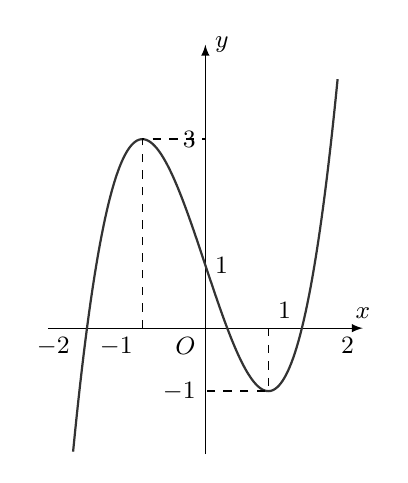
\begin{tikzpicture}[>=latex, scale=0.8]
    % Vẽ hệ trục tọa độ Ox, Oy
    \draw[->] (-2.5,0) -- (2.5,0) node[above] {\small $x$};
    \draw[->] (0,-2.0) -- (0,4.5) node[right] {\small $y$};
    \node[below left] at (0,0) {\small $O$};
    
    % Nhãn tọa độ
    \node[below left] at (-2,0) {\small $-2$};
    \node[below left] at (-1,0) {\small $-1$};
    \node[above right] at (1,0) {\small $1$};
    \node[below right] at (2,0) {\small $2$};
    \node[left] at (0,-1) {\small $-1$};
    \node[right] at (0,1) {\small $1$};
    \node[left] at (0,3) {\small $3$};
    
    % Đồ thị hàm bậc 3 chuẩn: y = x^3 - 3x + 1
    \draw[thick, color=black!80, samples=150, domain=-2.1:2.1] 
        plot (\x, {\x*\x*\x - 3*\x + 1}); 
        
    % Nét đứt gióng chuẩn tọa độ cực đại (-1; 3) và cực tiểu (1; -1)
    \draw[dashed, line width=0.5pt] (-1,0) -- (-1,3) -- (0,3);
    \draw[dashed, line width=0.5pt] (1,0) -- (1,-1) -- (0,-1);
\end{tikzpicture}
\end{center}}{%
\begin{tasks}(4)
\task \((-1;1)\).
\task \((-2;-1)\).
\task \((-1;2)\).
\task \((1;+\infty)\).
\end{tasks}
}

% ====== CÂU 24 (Câu 30 trong ảnh) ======
\questionLinesManual{0}{24}{Cho hàm số \( y = f(x) \) có đồ thị như hình vẽ bên.
\begin{center}
\begin{tikzpicture}[>=latex, scale=0.8]
    % Vẽ hệ trục tọa độ Ox, Oy
    \draw[->] (-3.5,0) -- (4.0,0) node[below] {\small $x$};
    \draw[->] (0,-4.8) -- (0,4.0) node[right] {\small $y$};
    \node[above left] at (0,0) {\small $O$};
    
    % Điền nhãn tọa độ trên trục chuẩn theo hình vẽ
    \node[above left] at (-2,0) {\small $-2$};
    \node[above left] at (1,0) {\small $1$};
    \node[below right] at (2,0) {\small $2$};
    \node[below] at (3,0) {\small $3$};
    \node[left] at (0,-1) {\small $-1$};
    \node[right] at (0,-4) {\small $-4$};
    
   % Nhánh trái (x <= 0): y = -x^3 - 3x^2
    \draw[thick, color=black!80, samples=100, domain=-3.2:0] 
        plot (\x, {-\x*\x*\x - 3*\x*\x}); 
        
   % Nhánh phải (x > 0): y = x^2 - 2x
    \draw[thick, color=black!80, samples=100, domain=0:3.15] 
        plot (\x, {\x*\x - 2*\x});
    % Các đường nét đứt gióng tọa độ chuẩn chỉnh theo hình vẽ
    \draw[dashed, line width=0.5pt] (-2, 0) -- (-2, -4) -- (0, -4);
    \draw[dashed, line width=0.5pt] (1, 0) -- (1, -1) -- (0, -1);
    \draw[dashed, line width=0.5pt] (3, 0) -- (3, 3) -- (0, 3);
\end{tikzpicture}
\end{center}
Hàm số đã cho nghịch biến trên khoảng nào?}{%
\begin{tasks}(4)
\task \((-1;0)\).
\task \((-2;-1)\).
\task \((0;1)\).
\task \((1;3)\).
\end{tasks}
}

% ====== CÂU 25 ======
\questionLinesManual{0}{25}{Cho hàm số \( f(x) \) liên tục trên \( \mathbb{R} \) và có đồ thị như hình vẽ bên. Khẳng định nào sau đây là đúng?
\begin{center}
\begin{tikzpicture}[>=latex, scale=1]
    % Hệ trục tọa độ
    \draw[->] (-2.5,0) -- (2.5,0) node[below] {\small $x$};
    \draw[->] (0,-2.5) -- (0,2.5) node[right] {\small $y$};
    \node[above left] at (0,0) {\small $O$};
    
    \draw[thick, color=black!80, samples=150, domain=-1.5:1.5] 
       plot (\x, {\x*\x*\x*\x - 2*\x*\x + 1});
    \node[below] at (-1,0) {\small $-1$};
    \node[below] at (1,0) {\small $1$};
    \node[above right] at (0,1) {\small $1$};
\end{tikzpicture}
\end{center}}{%
\begin{tasks}(2)
\task Hàm số đồng biến trên \((-\infty; 0)\) và \((0; +\infty)\).
\task Hàm số đồng biến trên \((-1; 0)\) và \((1; +\infty)\).
\task Hàm số đồng biến trên \((-1; 0) \cup (1; +\infty)\).
\task Hàm số đồng biến trên \((-\infty; -1) \cup (1; +\infty)\).
\end{tasks}
}

% ====== CÂU 26 ======
\questionLinesManual{0}{26}{Cho hàm số \( y = f(x) \) đồ thị hàm số như hình vẽ. Hàm số đồng biến trên khoảng nào?
\begin{center}
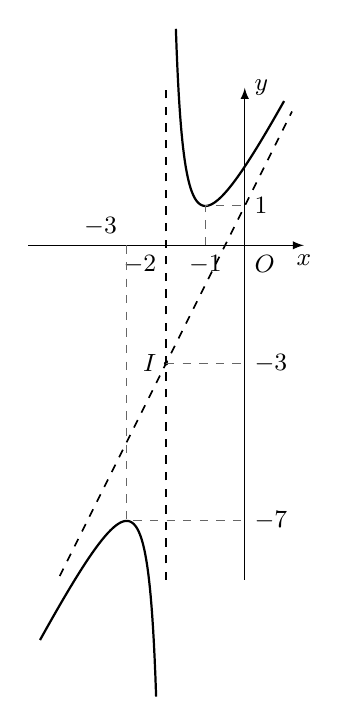
\begin{tikzpicture}[>=latex, scale=0.5]
    % Vẽ hệ trục tọa độ Ox, Oy màu đen
    \draw[->, black] (-5.5,0) -- (1.5,0) node[below] {\small $x$};
    \draw[->, black] (0,-8.5) -- (0,4.0) node[right] {\small $y$};
    \node[below right] at (0,0) {\small $O$};
    
    % Điền các nhãn tọa độ trên trục hoành và trục tung
    \node[above left] at (-3,0) {\small $-3$};
    \node[below left] at (-2,0) {\small $-2$};
    \node[below] at (-1,0) {\small $-1$};
    \node[right] at (0,1) {\small $1$};
    \node[right] at (0,-3) {\small $-3$};
    \node[right] at (0,-7) {\small $-7$};
    
    % Vẽ tiệm cận đứng (x = -2) và tiệm cận xiên (y = 2x + 1) bằng nét đứt màu đen
    \draw[dashed, black, line width=0.6pt] (-2,-8.5) -- (-2,4.0);
    \draw[dashed, black, line width=0.6pt, domain=-4.7:1.2] plot (\x, {2*\x + 1});
    \fill[black] (-2,-3) circle (1.5pt) node[left] {\small $I$}; % Tâm đối xứng I màu đen
    
    % VẼ ĐỒ THỊ MÀU ĐEN CHUẨN XÁC THEO HÀM SỐ: y = 2x + 1 + 2/(x + 2)
    % Nhánh trái (x < -2)
    \draw[thick, color=black, samples=150, domain=-5.2:-2.25] 
        plot (\x, {2*\x + 1 + 2/(\x + 2)});
        
    % Nhánh phải (x > -2)
    \draw[thick, color=black, samples=150, domain=-1.75:1.0] 
        plot (\x, {2*\x + 1 + 2/(\x + 2)});
        
    % Các đường nét đứt gióng tọa độ cực trị màu đen mảnh (light/thin)
    \draw[dashed, black!60, line width=0.4pt] (-1,0) -- (-1,1) -- (0,1);     % Cực tiểu (-1; 1)
    \draw[dashed, black!60, line width=0.4pt] (-3,0) -- (-3,-7) -- (0,-7);   % Cực đại (-3; -7)
    \draw[dashed, black!60, line width=0.4pt] (-2,-3) -- (0,-3);             % Cao độ của tâm I
\end{tikzpicture}
\end{center}}{%
\begin{tasks}(4)
\task \((-1; +\infty)\)
\task \((-\infty; -1)\)
\task \((-3; 0)\)
\task \((-2; -1)\)
\end{tasks}
}

% ====== CÂU 27 (Câu 4 trong ảnh) ======
\questionLinesManual{0}{27}{Cho hàm số \( y = x^3 - 3x^2 \). Mệnh đề nào dưới đây đúng?

\begin{tasks}(2)
\task Hàm số đồng biến trên khoảng \( (0; 2) \)
\task Hàm số nghịch biến trên khoảng \( (0; 2) \)
\task Hàm số nghịch biến trên khoảng \( (-\infty; 0) \)
\task Hàm số nghịch biến trên khoảng \( (2; +\infty) \)
\end{tasks}
}

% ====== CÂU 28 (Câu 5 trong ảnh) ======
\questionLinesManual{0}{28}{Hỏi hàm số \( y = 2x^4 + 1 \) đồng biến trên khoảng nào?
\begin{tasks}(4)
\task \( (-\infty; 0) \)
\task \( (-\infty; -\dfrac{1}{2}) \)
\task \( (0; +\infty) \)
\task \( (-\dfrac{1}{2}; +\infty) \)
\end{tasks}
}

% ====== CÂU 29 (Câu 6 trong ảnh) ======
\questionLinesManual{0}{29}{Cho hàm số \( y = f(x) \) có đạo hàm \( f'(x) = x^2 + 1 \), \( \forall x \in \mathbb{R} \). Mệnh đề nào dưới đây đúng?}{%
\begin{tasks}(2)
\task Hàm số nghịch biến trên khoảng \( (1; +\infty) \)
\task Hàm số nghịch biến trên khoảng \( (-1; 1) \)
\task Hàm số đồng biến trên khoảng \( (-\infty; +\infty) \)
\task Hàm số nghịch biến trên khoảng \( (-\infty; 0) \)
\end{tasks}
}

% ====== CÂU 30 (Câu 7 trong ảnh) ======
\questionLinesManual{0}{30}{Cho hàm số \( y = x^3 - 2x^2 + x + 1 \). Mệnh đề nào dưới đây đúng?}{%
\begin{tasks}(2)
\task Hàm số nghịch biến trên khoảng \( (1; +\infty) \)
\task Hàm số nghịch biến trên khoảng \( (-\dfrac{1}{3}; 1) \)
\task Hàm số nghịch biến trên khoảng \( (-\infty; -\dfrac{1}{3}) \)
\task Hàm số đồng biến trên khoảng \( (-\dfrac{1}{3}; 1) \)
\end{tasks}
}

% ====== CÂU 31 (Câu 8 trong ảnh) ======
\questionLinesManual{0}{31}{Cho hàm số \( y = x^4 - 2x^2 \). Mệnh đề nào dưới đây đúng?
\begin{tasks}(2)
\task Hàm số nghịch biến trên khoảng \((-\infty; -2)\)
\task Hàm số đồng biến trên khoảng \((-1; 1)\)
\task Hàm số nghịch biến trên khoảng \((-1; 1)\)
\task Hàm số đồng biến trên khoảng \((-\infty; -2)\)
\end{tasks}
}

% ====== CÂU 32 (Câu 10 trong ảnh) ======
\questionLinesManual{0}{32}{Cho hàm số \( y = x^3 + 3x + 2 \). Mệnh đề nào dưới đây là đúng?}{%
\begin{tasks}(1)
\task Hàm số nghịch biến trên khoảng \((-\infty; 0)\) và đồng biến trên khoảng \((0; +\infty)\)
\task Hàm số đồng biến trên khoảng \((-\infty; 0)\) và đồng biến trên khoảng \((0; +\infty)\)
\task Hàm số đồng biến trên khoảng \((-\infty; +\infty)\)
\task Hàm số nghịch biến trên khoảng \((-\infty; +\infty)\)
\end{tasks}
}

% ====== CÂU 33 (Câu 11 trong ảnh) ======
\questionLinesManual{0}{33}{Cho hàm số \( y = \sqrt{2x^2 + 1} \). Mệnh đề nào dưới đây đúng?}{%
\begin{tasks}(1)
\task Hàm số đồng biến trên khoảng \((0; +\infty)\)
\task Hàm số đồng biến trên khoảng \((-\infty; 0)\)
\task Hàm số nghịch biến trên khoảng \((0; +\infty)\)
\task Hàm số nghịch biến trên khoảng \((-1; 1)\)
\end{tasks}
}

% ====== CÂU 34 (Câu 12 trong ảnh) ======
\questionLinesManual{0}{34}{Cho hàm số \( y = \dfrac{x^3}{3} - x^2 + x + 2019 \). Mệnh đề nào dưới đây đúng?}{%
\begin{tasks}(1)
\task Hàm số đã cho đồng biến trên \( \mathbb{R} \).
\task Hàm số đã cho nghịch biến trên \( (-\infty; 1) \).
\task Hàm số đã cho đồng biến trên \( (-\infty; 1) \) và nghịch biến trên \( (1; +\infty) \).
\task Hàm số đã cho đồng biến trên \( (1; +\infty) \) và nghịch biến trên \( (-\infty; 1) \).
\end{tasks}
}

% ====== CÂU 35 (Câu 15 trong ảnh) ======
\questionLinesManual{0}{35}{Hàm số \( y = -x^3 + 3x^2 - 2 \) đồng biến trên khoảng

\begin{tasks}(4)
\task \( (0; 2) \)
\task \( (-\infty; 0) \)
\task \( (1; 4) \)
\task \( (4; +\infty) \)
\end{tasks}
}

% ====== CÂU 36 (Câu 16 trong ảnh) ======
\questionLinesManual{0}{36}{Hàm số \( y = x^4 - 4x^3 \) đồng biến trên khoảng

\begin{tasks}(4)
\task \( (-\infty; +\infty) \)
\task \( (3; +\infty) \)
\task \( (-1; +\infty) \)
\task \( (-\infty; 0) \)
\end{tasks}
}

% ====== CÂU 37 (Câu 18 trong ảnh) ======
\questionLinesManual{0}{37}{Cho hàm số \( y = f(x) \) liên tục trên \( \mathbb{R} \) và có đạo hàm  
\( f'(x) = (1 - x)^2 (x + 1)^3 (3 - x). \)  
Hàm số \( y = f(x) \) đồng biến trên khoảng nào dưới đây?}{%
\begin{tasks}(4)
\task \((-\infty; 1)\)
\task \((-\infty; -1)\)
\task \((1; 3)\)
\task \((3; +\infty)\)
\end{tasks}
}

% ====== CÂU 38 (Câu 19 trong ảnh) ======
\questionLinesManual{0}{38}{Cho hàm số \( y = \log_3 (x^2 - 2x + 3) \). Hàm số đồng biến trên khoảng nào sau đây?}{%
\begin{tasks}(4)
\task \((-\infty; 1)\)
\task \((-1; +\infty)\)
\task \((-\infty; -1)\)
\task \((1; +\infty)\)
\end{tasks}
}

% ====== CÂU 39 (Câu 26 trong ảnh) ======
\questionLinesManual{0}{39}{Cho hàm số \( y = f(x) \) có đạo hàm \( f'(x) = x(x - 2)^3 \), với mọi \( x \in \mathbb{R} \). Hàm số đã cho nghịch biến trên khoảng nào dưới đây?}{%
\begin{tasks}(4)
\task \((1; 3)\)
\task \((-1; 0)\)
\task \((0; 1)\)
\task \((-2; 0)\)
\end{tasks}
}

% ====== CÂU 40 (Câu 24 trong ảnh) ======
\questionLinesManual{0}{40}{Cho hàm \( y = \sqrt{x^2 - 6x + 5} \). Mệnh đề nào sau đây là đúng?}{%
\begin{tasks}(2)
\task Hàm số đồng biến trên khoảng \((5; +\infty)\)
\task Hàm số đồng biến trên khoảng \((3; +\infty)\)
\task Hàm số đồng biến trên khoảng \((-\infty; 1)\)
\task Hàm số nghịch biến trên khoảng \((-\infty; 3)\)
\end{tasks}
}

% ====== CÂU 41 (Câu 22 trong ảnh) ======
\questionLinesManual{0}{41}{Hàm số \( y = f(x) \) có đạo hàm \( y' = x^2 \). Mệnh đề nào sau đây đúng?}{%
\begin{tasks}(1)
\task Hàm số nghịch biến trên \( \mathbb{R} \)
\task Hàm số nghịch biến trên \((-\infty; 0)\) và đồng biến trên \((0; +\infty)\)
\task Hàm số đồng biến trên \( \mathbb{R} \)
\task Hàm số đồng biến trên \((-\infty; 0)\) và nghịch biến trên \((0; +\infty)\)
\end{tasks}
}

% ====== CÂU 42 (Câu 18 trong ảnh) ======
\questionLinesManual{0}{42}{Cho hàm số \( f(x) \) liên tục trên \( \mathbb{R} \) có đạo hàm  
\( f'(x) = (x+2)(x-1), \forall x \in \mathbb{R}. \) 
Hàm số đã cho nghịch biến trên khoảng nào sau đây?}{%
\begin{tasks}(4)
\task \((-2;1)\)
\task \((-\infty;-2)\)
\task \((-2;+\infty)\)
\task \((1;+\infty)\)
\end{tasks}
}

% ====== CÂU 43 (Câu 17 trong ảnh) ======
\questionLinesManual{0}{43}{Hàm số nào dưới đây đồng biến trên khoảng \((-\infty;+\infty)\)?}{%
\begin{tasks}(4)
\task \(y = -x^3 - 2x + 1\)
\task \(y = \frac{x-2}{x+1}\)
\task \(y = 3x^3 + 3x - 2\)
\task \(y = 2x^3 - 5x + 1\)
\end{tasks}
}

% ====== CÂU 44 (Câu 21 trong ảnh) ======
\questionLinesManual{0}{44}{Trong các hàm số cho dưới đây, hàm số nào đồng biến trên \( \mathbb{R} \)?}{%
\begin{tasks}(4)
\task \(y = \left(\dfrac{2024}{2025}\right)^x\)
\task \(y = \log_{2025}x\)
\task \(y = \ln x\)
\task \(y = e^x\)
\end{tasks}
}

% ====== CÂU 45 (Câu 25 trong ảnh) ======
\questionLinesManual{0}{45}{Hàm số nào sau đây nghịch biến trên các khoảng xác định của nó?}{%
\begin{tasks}(4)
\task \(y = e^{-x}\)
\task \(y = \log_{\sqrt{3}}x\)
\task \(y = (\sqrt{2})^x\)
\task \(y = \ln x\)
\end{tasks}
}

% ====== CÂU 46 (Câu 26 trong ảnh) ======
\questionLinesManual{0}{46}{Hàm số nào dưới đây nghịch biến trên \((-\infty;+\infty)\)?}{%
\begin{tasks}(4)
\task \(y = \ln x\)
\task \(y = \log_{\frac{1}{7}}x\)
\task \(y = \left(\dfrac{\pi}{6}\right)^x\)
\task \(y = e^x\)
\end{tasks}
}

% ====== CÂU 47 (Câu 14 trong ảnh) ======
\questionLinesManual{0}{47}{Cho hàm số \( y = f(x) \) xác định, có đạo hàm trên \( \mathbb{R} \) và \( f'(x) \) có đồ thị như hình vẽ bên dưới
\begin{center}
\begin{tikzpicture}[>=latex, scale=1]
    % Hệ trục tọa độ
    \draw[->] (-4.5,0) -- (4.5,0) node[below] {\small $x$};
    \draw[->] (0,-3.5) -- (0,3.5) node[right] {\small $y$};
    \node[above left] at (0,0) {\small $O$};
    
    % Vẽ đồ thị f'(x) là parabol hướng lên có nghiệm tại x = -3 và x = 1
    \draw[thick, color=black!80, samples=150, domain=-3.2:0.7] 
       plot (\x, {-0.5*(\x*\x*\x*\x + 5*\x*\x*\x + 6*\x*\x)}); 
        
    % Ký hiệu tên hàm số f'(x) ở góc phải bên dưới
    \node[right] at (0.5,-3.0) {\small $f'(x)$};
    
    % Đánh dấu các điểm trên trục Ox
    \node[below] at (-3,0) {\small $-3$};
    \node[below] at (1,0) {\small $1$};
    \node[above right] at (-2,0) {\small $-2$};
\end{tikzpicture}
\end{center}
Mệnh đề nào sau đây đúng?}{%
\begin{tasks}(1)
\task Hàm số \( y = f(x) \) nghịch biến trên khoảng \( \left( -\dfrac{5}{2}; -2 \right] \).
\task Hàm số \( y = f(x) \) nghịch biến trên khoảng \( (-2; +\infty) \).
\task Hàm số \( y = f(x) \) đồng biến trên khoảng \( (-\infty; -3) \).
\task Hàm số \( y = f(x) \) đồng biến trên khoảng \( \left( -\dfrac{1}{2}; 0 \right] \).
\end{tasks}
}

% ====== CÂU 48 (Câu 16 trong ảnh) ======
\questionLinesManual{0}{48}{Cho hàm số \( y = f(x) \) có đạo hàm trên \( \mathbb{R} \) và đồ thị của hàm số \( y = f'(x) \) như hình vẽ.
\begin{center}
\begin{tikzpicture}[>=latex, scale=0.8]
    % Hệ trục tọa độ
    \draw[->] (-4.5,0) -- (4.5,0) node[below] {\small $x$};
    \draw[->] (0,-3.5) -- (0,5) node[right] {\small $y$};
    \node[above left] at (0,0) {\small $O$};
    
    % Vẽ đồ thị f'(x) là parabol hướng lên có nghiệm tại x = -2 và x = 2
    \draw[thick, color=black!80, samples=150, domain=-2.2:2.1] 
        plot (\x, {(\x*\x*\x - 3*\x + 2)});
    
    % Đánh dấu các điểm trên trục Ox
    \draw[dashed] (-1,0) -- (-1,4);
    \draw[dashed] (-1,4) -- (0,4);
    \node[below] at (-2,0) {\small $-2$};
    \node[below] at (-1,0) {\small $-1$};
    \node[below] at (1,0) {\small $1$};
     \node[right] at (0,4) {\small $4$};
\end{tikzpicture}
\end{center}
Hàm số \( g(x) = f(x) - 2 \) nghịch biến trên khoảng nào trong các khoảng sau?}{%
\begin{tasks}(4)
\task \((-1; 1)\)
\task \((-\infty; -2)\)
\task \((2; +\infty)\)
\task \((1; 3)\)
\end{tasks}
}

% ====== CÂU 49 (Câu 22 trong ảnh) ======
\questionLinesManual{0}{49}{Cho hàm số \( y = f(x) \) xác định, có đạo hàm trên \( \mathbb{R} \) và \( f'(x) \) có đồ thị như hình vẽ bên dưới
\begin{center}
\begin{tikzpicture}[>=latex, scale=0.8]
    % Hệ trục tọa độ
    \draw[->] (-4.5,0) -- (4.5,0) node[below] {\small $x$};
    \draw[->] (0,-5) -- (0,3.5) node[right] {\small $y$};
    \node[above left] at (0,0) {\small $O$};
    
    % Vẽ đồ thị f'(x) là parabol hướng lên có nghiệm tại x = -3, x = -1, x = 2
    \draw[thick, color=black!80, samples=150, domain=-2.2:2.3] 
       plot (\x, {-0.5*\x*\x*\x*\x + 0.5*\x*\x*\x + 3*\x*\x - 2*\x - 4});
    
    % Đánh dấu các điểm trên trục Ox
    \node[above left] at (-2,0) {\small $-2$};
    \node[above left] at (-1,0) {\small $-1$};
    \node[left] at (0,-4) {\small $-4$};
    \node[above] at (2,0) {\small $2$};
\end{tikzpicture}
\end{center}
Mệnh đề nào sau đây sai?}{%
\begin{tasks}(1)
\task Hàm số \( y = f(x) \) nghịch biến trên khoảng \( \left( -\dfrac{1}{2}; 0 \right) \).
\task Hàm số \( y = f(x) \) nghịch biến trên khoảng \( \left( -\dfrac{5}{2}; -2 \right) \).
\task Hàm số \( y = f(x) \) đồng biến trên khoảng \( (-2; +\infty) \).
\task Hàm số \( y = f(x) \) nghịch biến trên khoảng \( (1; 2) \).
\end{tasks}
}
% ====== CÂU 50 (Câu 27 trong ảnh) ======
\questionLinesManual{0}{50}{Cho hàm số \( y = f(x) \) có đạo hàm trên \( \mathbb{R} \) thỏa mãn \( f'(x) > 0, \forall x \in (-1; 0) \) và \( f'(x) < 0, \forall x \in (0; 1) \). Khẳng định nào sau đây là đúng?}{%
\begin{tasks}(1)
\task Hàm số \( f(x) \) nghịch biến trên khoảng \( (-1; 0) \) và đồng biến trên khoảng \( (0; 1) \).
\task Hàm số \( f(x) \) đồng biến trên các khoảng \( (-1; 0) \) và \( (0; 1) \).
\task Hàm số \( f(x) \) nghịch biến trên các khoảng \( (-1; 0) \) và \( (0; 1) \).
\task Hàm số \( f(x) \) đồng biến trên khoảng \( (-1; 0) \) và nghịch biến trên khoảng \( (0; 1) \).
\end{tasks}
}

% ====== CÂU 51 (Câu 30 trong ảnh) ======
\questionLinesManual{0}{51}{Cho hàm số \( y = f(x) \) xác định với mọi \( x \neq 0 \) và có bảng xét dấu \( f'(x) \) như hình vẽ dưới đây.
\begin{center}
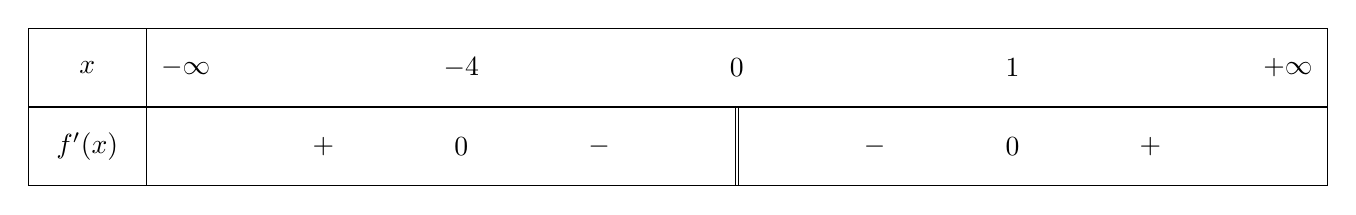
\begin{tikzpicture}
\tkzTabInit[color, lgt=1.5, espcl=3.5]
{$x$ / 1, $f'(x)$ / 1}
{$-\infty$, $-4$, $0$, $1$, $+\infty$}
\tkzTabLine{ , +, 0, -, d, -, 0, + }
\end{tikzpicture}
\end{center}
Hàm số \( f(x) \) nghịch biến trên khoảng nào trong các khoảng sau?}{%
\begin{tasks}(4)
\task \( (1; +\infty) \)
\task \( (-4; +\infty) \)
\task \( (-4; 1) \)
\task \( (-4; 0) \)
\end{tasks}
}

% ====== CÂU 52 (Đúng/Sai) ======
\questionTrueFalse{0}{52}{Cho hàm số \( y = f(x) \) có bảng xét dấu đạo hàm như sau:
\begin{center}
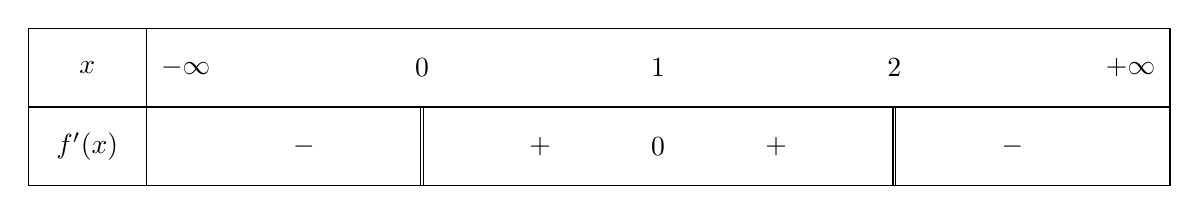
\begin{tikzpicture}
\tkzTabInit[color, lgt=1.5, espcl=3]
{$x$ / 1, $f'(x)$ / 1}
{$-\infty$, $0$, $1$, $2$, $+\infty$}
\tkzTabLine{ , -, d, +, 0, +, d, - }
\end{tikzpicture}
\end{center}}{
    \textbf{a)} & Hàm số đồng biến trên khoảng \( (0; 2) \). 
    & \textcolor{amberorange}{$\bigcirc$} & \textcolor{amberorange}{$\bigcirc$} \\ \hline
    \textbf{b)} & Hàm số đồng biến trên khoảng \( (1; 2) \).
    & \textcolor{amberorange}{$\bigcirc$} & \textcolor{amberorange}{$\bigcirc$} \\ \hline
    \textbf{c)} & Hàm số nghịch biến trên khoảng \( (-\infty; +\infty) \).
     & \textcolor{amberorange}{$\bigcirc$} & \textcolor{amberorange}{$\bigcirc$} \\ \hline
    \textbf{d)} & Hàm số nghịch biến trên các khoảng \( (-\infty; 0) \) và \( (2; +\infty) \). 
    & \textcolor{amberorange}{$\bigcirc$} & \textcolor{amberorange}{$\bigcirc$} \\
}

% ====== CÂU 53 (Đúng/Sai) ======
\questionTrueFalse{0}{53}{Cho hàm số \( y = \dfrac{x^3}{3} - 2x^2 + 3x - 1 \).}{
    \textbf{a)} & Hàm số nghịch biến trên khoảng \( (1; 3) \). 
    & \textcolor{amberorange}{$\bigcirc$} & \textcolor{amberorange}{$\bigcirc$} \\ \hline
    \textbf{b)} & Hàm số nghịch biến trên khoảng \( (-\infty; 1) \).
    & \textcolor{amberorange}{$\bigcirc$} & \textcolor{amberorange}{$\bigcirc$} \\ \hline
    \textbf{c)} & Hàm số đồng biến trên khoảng \( (1; 3) \).
     & \textcolor{amberorange}{$\bigcirc$} & \textcolor{amberorange}{$\bigcirc$} \\ \hline
    \textbf{d)} & Hàm số đồng biến trên các khoảng \( (-\infty; 1) \) và \( (3; +\infty) \). 
    & \textcolor{amberorange}{$\bigcirc$} & \textcolor{amberorange}{$\bigcirc$} \\
}

% ====== CÂU 54 (Đúng/Sai) ======
\questionTrueFalse{0}{54}{Cho hàm số \( f(x) = x^2 e^x \).}{
    \textbf{a)} & Hàm số đồng biến trên khoảng \( (-\infty; -2) \). 
    & \textcolor{amberorange}{$\bigcirc$} & \textcolor{amberorange}{$\bigcirc$} \\ \hline
    \textbf{b)} & Hàm số nghịch biến trên khoảng \( (0; +\infty) \).
    & \textcolor{amberorange}{$\bigcirc$} & \textcolor{amberorange}{$\bigcirc$} \\ \hline
    \textbf{c)} & Hàm số nghịch biến trên khoảng \( (0; 2) \).
     & \textcolor{amberorange}{$\bigcirc$} & \textcolor{amberorange}{$\bigcirc$} \\ \hline
    \textbf{d)} & Hàm số nghịch biến trên khoảng \( (-2; 0) \). 
    & \textcolor{amberorange}{$\bigcirc$} & \textcolor{amberorange}{$\bigcirc$} \\
}

% ====== CÂU 55 (Câu 4) ======
\questionTrueFalse{0}{55}{Cho hàm số \( f(x) \) có đạo hàm \( f'(x) = x(x-3)^3 \) với mọi \( x \in \mathbb{R} \). }{
    \textbf{a)} & Hàm số \( f(x) \) đồng biến trên khoảng \((-1; 0)\). 
    & \textcolor{amberorange}{$\bigcirc$} & \textcolor{amberorange}{$\bigcirc$} \\ \hline
    \textbf{b)} & Hàm số \( f(x) \) đồng biến trên khoảng \((-2; 1)\).
    & \textcolor{amberorange}{$\bigcirc$} & \textcolor{amberorange}{$\bigcirc$} \\ \hline
    \textbf{c)} & \( f(1) > f(2) \).
    & \textcolor{amberorange}{$\bigcirc$} & \textcolor{amberorange}{$\bigcirc$} \\ \hline
    \textbf{d)} & \( f(5) < f(4) \).
    & \textcolor{amberorange}{$\bigcirc$} & \textcolor{amberorange}{$\bigcirc$} \\
}

% ====== CÂU 56 (Câu 5) ======
\questionTrueFalse{0}{56}{Cho hàm số \( y = f(x) \) có đạo hàm trên \( \mathbb{R} \) và đồ thị hàm số \( y = f'(x) \) như hình.
\begin{center}
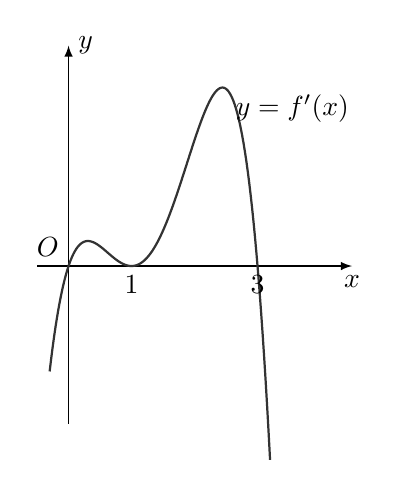
\begin{tikzpicture}[>=latex, scale=0.8]
    % Hệ trục tọa độ
    \draw[->] (-0.5,0) -- (4.5,0) node[below] {$x$};
    \draw[->] (0,-2.5) -- (0,3.5) node[right] {$y$};
    \node[above left] at (0,0) {$O$};
    
    % Vẽ đồ thị f'(x) là parabol hướng lên có nghiệm tại x = 0, x = 1, x = 3
    \draw[thick, color=black!80, samples=150, domain=-0.3:3.2] 
         plot (\x, {-\x*\x*\x*\x + 5*\x*\x*\x - 7*\x*\x + 3*\x}); 
        
    % Đánh dấu các điểm trên trục Ox
    \node[below] at (1,0) {$1$};
    \node[below] at (3,0) {$3$};
    \node[right] at (2.5,2.5) {$y = f'(x)$};
\end{tikzpicture}
\end{center}}{
    \textbf{a)} & \( f'(x) = 0 \) khi \( x = 0, x = 1, x = 3 \). 
    & \textcolor{amberorange}{$\bigcirc$} & \textcolor{amberorange}{$\bigcirc$} \\ \hline
    \textbf{b)} & Hàm số \( y = f(x) \) đồng biến trên khoảng \((-\infty; 0)\).
    & \textcolor{amberorange}{$\bigcirc$} & \textcolor{amberorange}{$\bigcirc$} \\ \hline
    \textbf{c)} & \( f'(x) > 0 \) khi \( x \in (0; 3) \).
    & \textcolor{amberorange}{$\bigcirc$} & \textcolor{amberorange}{$\bigcirc$} \\ \hline
    \textbf{d)} & Hàm số \( y = f(x) \) đồng biến trên khoảng \((0; 3)\).
    & \textcolor{amberorange}{$\bigcirc$} & \textcolor{amberorange}{$\bigcirc$} \\
}

% ====== CÂU 57 (Câu 6) ======
\questionTrueFalse{0}{57}{Cho hàm số bậc bốn \( y = f(x) \) có dạng đồ thị như hình vẽ.
\begin{center}
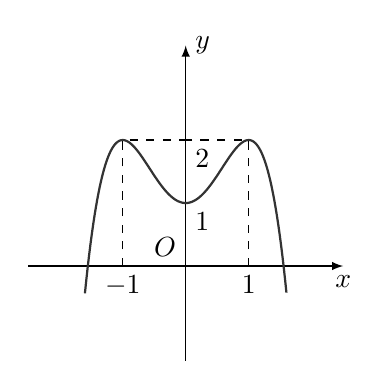
\begin{tikzpicture}[>=latex, scale=0.8]
    % Hệ trục tọa độ
    \draw[->] (-2.5,0) -- (2.5,0) node[below] {$x$};
    \draw[->] (0,-1.5) -- (0,3.5) node[right] {$y$};
    \node[above left] at (0,0) {$O$};
    
    % Vẽ đồ thị hàm bậc 4 trùng phương y = x^4 - 2x^2
    \draw[thick, color=black!80, samples=150, domain=-1.6:1.6] 
        plot (\x, {-\x*\x*\x*\x + 2*\x*\x + 1});
    
    % Đánh dấu các điểm
    \draw[dashed] (-1,0) -- (-1,2) -- (0,2);
    \draw[dashed] (1,0) -- (1,2) -- (0,2);
    \node[below] at (-1,0) {$-1$};
    \node[below] at (1,0) {$1$};
    \node[below right] at (0,2) {$2$};
    \node[below right] at (0,1) {$1$};
\end{tikzpicture}
\end{center}}{
    \textbf{a)} & Hàm số đồng biến trên khoảng \( (1; 2) \). 
    & \textcolor{amberorange}{$\bigcirc$} & \textcolor{amberorange}{$\bigcirc$} \\ \hline
    \textbf{b)} & \( f\left(\frac{1}{2}\right) > 0 \).
    & \textcolor{amberorange}{$\bigcirc$} & \textcolor{amberorange}{$\bigcirc$} \\ \hline
    \textbf{c)} & Hàm số nghịch biến trên khoảng \( (2; +\infty) \).
    & \textcolor{amberorange}{$\bigcirc$} & \textcolor{amberorange}{$\bigcirc$} \\ \hline
    \textbf{d)} & Hàm số nghịch biến trên khoảng \( (-1; 0) \).
    & \textcolor{amberorange}{$\bigcirc$} & \textcolor{amberorange}{$\bigcirc$} \\
}

% ====== CÂU 58 (Câu 7) ======
\questionTrueFalse{0}{58}{Cho hàm số \( y = f(x) \) liên tục trên \( \mathbb{R} \) và có bảng biến thiên như sau:
 \begin{center}
        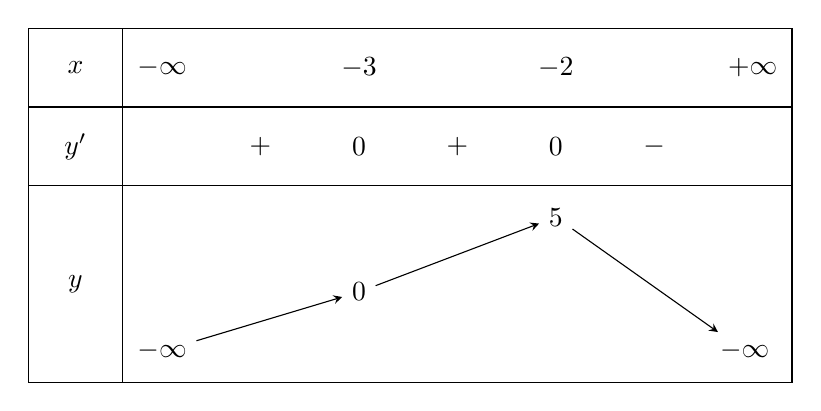
\begin{tikzpicture}[>=stealth]
            \tkzTabInit[nocadre=false,lgt=1.2,espcl=2.5]
            {$x$ / 1, $y'$ / 1, $y$ / 2.5}
            {$-\infty$, $-3$, $-2$, $+\infty$}
            \tkzTabLine{ , +, 0, +, 0, -, }
            
            
            \node (y1) at (1.7, -4.1) {$-\infty$};
            \node (y2) at (4.2, -3.35) {$0$};
            \node (y3) at (6.7, -2.4) {$5$};
            \node (y4) at (9.1, -4.1) {$-\infty$};
            
            \draw[->] (y1) -- (y2);
            \draw[->] (y2) -- (y3);
            \draw[->] (y3) -- (y4);
        \end{tikzpicture}
    \end{center}}{
    \textbf{a)} & Hàm số đã cho đồng biến trên các khoảng \((-\infty; -3)\) và \((-3; -2)\).
    & \textcolor{amberorange}{$\bigcirc$} & \textcolor{amberorange}{$\bigcirc$} \\ \hline
    \textbf{b)} & Hàm số đã cho đồng biến trên khoảng \((-\infty; 5)\).
    & \textcolor{amberorange}{$\bigcirc$} & \textcolor{amberorange}{$\bigcirc$} \\ \hline
    \textbf{c)} & Hàm số đã cho nghịch biến trên khoảng \((-2; +\infty)\).
    & \textcolor{amberorange}{$\bigcirc$} & \textcolor{amberorange}{$\bigcirc$} \\ \hline
    \textbf{d)} & Hàm số đã cho đồng biến trên khoảng \((-\infty; -2)\).
    & \textcolor{amberorange}{$\bigcirc$} & \textcolor{amberorange}{$\bigcirc$} \\
}

% ====== CÂU 59 (Câu 8) ======
\questionTrueFalse{0}{59}{Cho hàm số \( f(x) \) có bảng xét dấu đạo hàm như sau:
\begin{center}
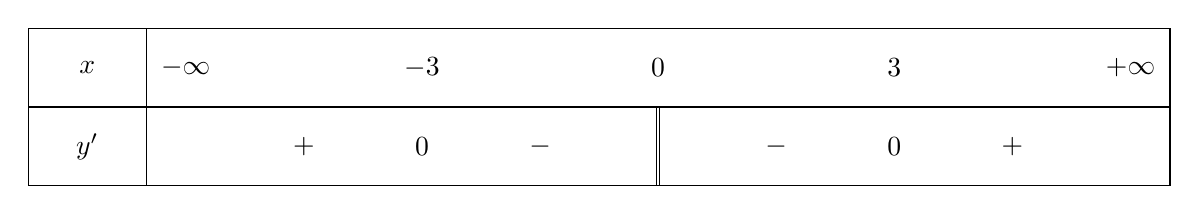
\begin{tikzpicture}
\tkzTabInit[color, lgt=1.5, espcl=3]
{$x$ / 1, $y'$ / 1}
{$-\infty$, $-3$, $0$, $3$, $+\infty$}
\tkzTabLine{ , +, 0, -, d, -, 0, + }
\end{tikzpicture}
\end{center}}{
    \textbf{a)} & Hàm số đồng biến trên khoảng \((-3; 0)\).
    & \textcolor{amberorange}{$\bigcirc$} & \textcolor{amberorange}{$\bigcirc$} \\ \hline
    \textbf{b)} & Hàm số nghịch biến trên khoảng \((0; 3)\).
    & \textcolor{amberorange}{$\bigcirc$} & \textcolor{amberorange}{$\bigcirc$} \\ \hline
    \textbf{c)} & Hàm số đồng biến trên khoảng \((-\infty; 0)\).
    & \textcolor{amberorange}{$\bigcirc$} & \textcolor{amberorange}{$\bigcirc$} \\ \hline
    \textbf{d)} & Hàm số nghịch biến trên khoảng \((-\infty; -3)\).
    & \textcolor{amberorange}{$\bigcirc$} & \textcolor{amberorange}{$\bigcirc$} \\
}

% ====== CÂU 60 (Câu 9) ======
\questionTrueFalse{0}{60}{Cho hàm số \( y = f(x) \) có đồ thị như hình vẽ bên.
\begin{center}
\begin{tikzpicture}[>=latex, scale=0.8]
    % Hệ trục tọa độ
    \draw[->] (-3,0) -- (4,0) node[below] {$x$};
    \draw[->] (0,-3.5) -- (0,4.5) node[right] {$y$};
    \node[below left] at (0,0) {$O$};
    
    % Nhãn tọa độ
    \node[below] at (-1,0) {$-1$};
    \node[above] at (2,0) {$2$};
    \node[left] at (0,3) {$3$};
    \node[left] at (0,-3) {$-3$};
    
    % Vẽ đồ thị hàm bậc 3 y = -x^3 + 3x + 3
    \draw[thick, color=black!80, samples=150, domain=-1.5:2.5] 
        plot (\x, {(9*\x*\x*\x*\x - 12*\x*\x*\x - 36*\x*\x)/16 + 3});
    
    % Đường nét đứt
    \draw[dashed, line width=0.5pt] (-1,0) -- (-1,2);
    \draw[dashed, line width=0.5pt] (2,0) -- (2,-3) -- (0,-3);
\end{tikzpicture}
\end{center}}{
    \textbf{a)} & Đồ thị hàm số cắt trục tung tại điểm có tung độ bằng 3.
    & \textcolor{amberorange}{$\bigcirc$} & \textcolor{amberorange}{$\bigcirc$} \\ \hline
    \textbf{b)} & Hàm số nghịch biến trên khoảng \((-3; 0)\).
    & \textcolor{amberorange}{$\bigcirc$} & \textcolor{amberorange}{$\bigcirc$} \\ \hline
    \textbf{c)} & Đồng biến trên khoảng \((-1; 0)\).
    & \textcolor{amberorange}{$\bigcirc$} & \textcolor{amberorange}{$\bigcirc$} \\ \hline
    \textbf{d)} & Nghịch biến trên khoảng \((0; 3)\).
    & \textcolor{amberorange}{$\bigcirc$} & \textcolor{amberorange}{$\bigcirc$} \\
}

% ====== CÂU 61 (Câu 10) ======
\questionTrueFalse{0}{61}{Cho hàm số \( y = f(x) \) đồng biến trên khoảng \( (a; b) \). Khi đó:}{
    \textbf{a)} & Hàm số \( y = f(x+1) \) đồng biến trên \( (a; b) \).
    & \textcolor{amberorange}{$\bigcirc$} & \textcolor{amberorange}{$\bigcirc$} \\ \hline
    \textbf{b)} & Hàm số \( y = -f(x) - 1 \) nghịch biến trên \( (a; b) \).
    & \textcolor{amberorange}{$\bigcirc$} & \textcolor{amberorange}{$\bigcirc$} \\ \hline
    \textbf{c)} & Hàm số \( y = -f(x) \) nghịch biến trên \( (a; b) \).
    & \textcolor{amberorange}{$\bigcirc$} & \textcolor{amberorange}{$\bigcirc$} \\ \hline
    \textbf{d)} & Hàm số \( y = f(x) + 1 \) đồng biến trên \( (a; b) \).
    & \textcolor{amberorange}{$\bigcirc$} & \textcolor{amberorange}{$\bigcirc$} \\
}

% ====== CÂU 62 (Câu 11) ======
\questionTrueFalse{0}{62}{Giả sử hàm số \( (C): y = f(x) \) nghịch biến trên khoảng \( K \) và hàm số \( (C'): y = g(x) \) đồng biến trên khoảng \( K \). Khi đó:}{
    \textbf{a)} & Hàm số \( f(x) + g(x) \) đồng biến trên khoảng \( K \).
    & \textcolor{amberorange}{$\bigcirc$} & \textcolor{amberorange}{$\bigcirc$} \\ \hline
    \textbf{b)} & Hàm số \( f(x) - g(x) \) nghịch biến trên khoảng \( K \).
    & \textcolor{amberorange}{$\bigcirc$} & \textcolor{amberorange}{$\bigcirc$} \\ \hline
    \textbf{c)} & Hàm số \( f(x)g(x) \) nghịch biến trên khoảng \( K \).
    & \textcolor{amberorange}{$\bigcirc$} & \textcolor{amberorange}{$\bigcirc$} \\ \hline
    \textbf{d)} & Đồ thị của hàm số \( (C) \) và \( (C') \) có đúng một điểm chung.
    & \textcolor{amberorange}{$\bigcirc$} & \textcolor{amberorange}{$\bigcirc$} \\
}

% ====== CÂU 63 (Câu 12) ======
\questionTrueFalse{0}{63}{Cho hàm số \( y = \sqrt{x^3 - 3x} \). Khi đó:}{
    \textbf{a)} & Tập xác định \( D = [-\sqrt{3}; 0] \cup [\sqrt{3}; +\infty) \).
    & \textcolor{amberorange}{$\bigcirc$} & \textcolor{amberorange}{$\bigcirc$} \\ \hline
    \textbf{b)} & Hàm số nghịch biến trên \((-1; 1)\).
    & \textcolor{amberorange}{$\bigcirc$} & \textcolor{amberorange}{$\bigcirc$} \\ \hline
    \textbf{c)} & Hàm số nghịch biến trên các khoảng \((-1; 0)\) và \((0; 1)\).
    & \textcolor{amberorange}{$\bigcirc$} & \textcolor{amberorange}{$\bigcirc$} \\ \hline
    \textbf{d)} & Hàm số đồng biến trên khoảng \((\sqrt{3}; +\infty)\).
    & \textcolor{amberorange}{$\bigcirc$} & \textcolor{amberorange}{$\bigcirc$} \\
}


\end{document}